\documentclass[11pt]{article}

% Packages
\usepackage[a4paper,margin=1in]{geometry}
\usepackage{amsmath,amssymb,amsthm,mathtools}
\usepackage[shortlabels]{enumitem}
\usepackage{hyperref}
\usepackage{tikz}
\usepackage{microtype}
\usepackage{natbib}
\usepackage{booktabs}
\usepackage{bbm}

\usepackage{xcolor}
\newcommand{\fixme}[1]{\textcolor{red}{Note to self: #1}}

\newcommand{\overbar}[1]{\mkern 1.5mu\overline{\mkern-1.5mu#1\mkern-1.5mu}\mkern 1.5mu}


% TikZ setup
\usetikzlibrary{arrows.meta,positioning,calc,decorations.pathreplacing}
\tikzset{
  >=Latex,
  doc/.style = {draw, rounded corners, inner sep=3pt, align=center, minimum width=1.2cm},
  sum/.style = {draw, rounded corners, inner sep=3pt, align=center, fill=blue!5},
  op/.style  = {inner sep=1pt, font=\small, align=center},
  plus/.style={circle, draw, inner sep=0pt, minimum size=14pt, font=\bfseries},
  every node/.style = {font=\small}
}

% Theorem environments
\newtheorem{definition}{Definition}
\newtheorem{assumption}{Assumption}
\newtheorem{lemma}{Lemma}
\newtheorem{proposition}{Proposition}
\newtheorem{theorem}{Theorem}
\newtheorem{remark}{Remark}
\newtheorem{example}{Example}
\newtheorem{corollary}{Corollary}

% Notation
\newcommand{\Strings}{\mathcal{X}}       % all finite strings (kleene closure)

\newcommand{\Y}{\mathcal{Y}}               % oracle output space
\newcommand{\Z}{\mathcal{Z}}               % model output space
\newcommand{\A}{\mathcal{A}}               % action space
\newcommand{\eps}{\varepsilon}             % empty string
\newcommand{\fstar}{f^*}               % oracle function
\newcommand{\fhat}{\hat{f}}               % oracle function
\newcommand{\sstar}{S^\star}               % supervision function
\newcommand{\Gstar}{\mathcal{G}^\star}     % set of f*-sufficient summarizers
\newcommand{\Prob}{\mathbb{P}}
\newcommand{\E}{\mathbb{E}}
\newcommand{\TV}{\mathrm{TV}}              % total variation

\newcommand{\concat}{\oplus}                    % concatenation operator

% \newcommand{\concat}{+}                     % concatenation operator

\newcommand{\metric}{d_{\Y}}

\newcommand{\lawtag}[1]{\tag{L#1}\label{eq:leaf_law#1}}


%  --  Notation fixes and measure-theoretic helpers  -- 
\newcommand{\emptystr}{\varnothing}              % empty string (identity element)
\renewcommand{\eps}{\varepsilon}                 % epsilon now only for scalars

\newcommand{\R}{\mathbb{R}}
% Probability kernels and test functions
\newcommand{\calP}{\mathcal{P}}
\newcommand{\Law}{\rho}
\newcommand{\TVnorm}[1]{\left\| #1 \right\|_{\mathrm{TV}}}
\newcommand{\ang}[2]{\left\langle #1,\ #2 \right\rangle}  % \langle test, measure \rangle

% Reduction function
\newcommand{\reduce}{\text{Reduce}}
% Randomness
\newcommand{\reduceg}{\reduce_g}

\newcommand{\Eg}{\E_g}     % expectation over summarizer randomness only

\newcommand{\congruence}{\textnormal{Congruence}}
\newcommand{\tre}{\textnormal{TRE}}

\title{Hierarchical Summarization with Oracle-Preserving Guarantees:\\
Aligning Human Preferences with Data Extraction Pipelines}

\author{Mitchell Linegar}
\date{}

\begin{document}
\maketitle

\begin{abstract}
We study how to turn very long documents into task‑relevant signals without losing what researchers actually care about. In practice, pipelines split a document into blocks, summarize each, and merge summaries up a tree. We give a local, auditable framework that says exactly when this hierarchical summarization is faithful to the intended task: treat the task value as an oracle, and enforce three checks only on the operations the hierarchy really executes: single‑block sufficiency at the leaves, agreement between the two natural routes at realized merges, and stability when re‑summarizing strings already in summary form. These local checks are enough to preserve the task value in expectation for any partition and for any merge schedule whose realized nodes pass the audit; extra normalization rounds remain inert. No global algebra is required (a global variant is provided for context, but not needed for guarantees). We also give an operational audit that estimates leaf, merge, and on‑range distortions and composes them additively into a single deployment‑level error budget. Finally, when supervision and pairwise preferences depend on inputs only through the task value, training Direct Preference Optimization on oracle‑preserving summaries attains the same population optimum as training on full documents; when preservation is approximate, the gap is quantitatively controlled by the audited empirical distortion.\footnote{Previous versions of this work have benefited from conversations with Mitchell Bosley, Yimeng Li, Patrick Brandt, Danny Ebanks, Matthew Estes, and Ransi Clark, as well as feedback from discussants at MPSA, the Texas Methods Meeting, and the Stories that Win Conference at Washington University in St. Louis.}
\end{abstract}

Social scientists increasingly rely on large, unstructured text corpora as primary data sources. From parliamentary debates to news coverage of protest events, from legal opinions to social media streams, the ability to turn documents into structured, analyzable signals has become central to empirical research. Yet the sheer size of these corpora, combined with the finite context windows of current large language models (LLMs), imposes severe constraints. Standard transformer models cannot ingest book-length documents or year-long Twitter feeds in a single forward pass. In practice, researchers and engineers resort to hierarchical strategies: segment long documents into blocks, summarize each, and then merge summaries upward into a tree. This pragmatic workaround is now ubiquitous, but it raises a practical question: when do such recursive summaries retain the information the task actually requires?

We answer this question by developing a framework for \emph{oracle-preserving} summarization. The starting point is simple: for each document there is a task value the researcher cares about—whether an event is reported, who did what to whom and where, or how many distinct events occurred. Hierarchical preprocessing is acceptable only if it leaves that value unchanged for the purposes of analysis and learning. To make this auditable, we focus on three local properties that are stated and checked on the very operations a deployed hierarchy performs: single-block sufficiency at the leaves; agreement between the two natural routes at each realized merge (summarize children, concatenate, summarize versus concatenate the underlying strings and summarize once); and stability when re‑summarizing strings that are already in summary form. These conditions are deliberately modest: they do not assume a global algebra for merges, and they allow stochastic summarizers whose internal randomness interacts with the realized schedule.

The first payoff is processing invariance under genuinely local hypotheses. For any fixed partition of a document, a single hierarchical pass preserves the task value in expectation for every binary merge tree \emph{whose realized leaves and internal nodes satisfy the local checks}. In particular, balanced trees and daisy‑chain schedules agree whenever each passes its own audit. The same logic extends to the common “fold‑of‑folds’’ schedules used for latency and cost, provided the local checks are enforced at the realized merges across both levels. When systems apply extra normalization rounds for consistency, the on‑range stability condition ensures that re‑summarization is inert in expectation, so repeated passes do not drift the task value.

The second payoff is a clean connection to learning. We consider supervision that depends on documents only through their task value, a common factorization that covers proper scoring, many coding tasks, and Bradley–Terry–Luce models for pairwise preferences. Under this assumption, training on oracle‑preserving summaries is information‑equivalent to training on full documents for linearly aggregated risks. Specializing to Direct Preference Optimization (DPO), if the hierarchy preserves the task value along the realized tree, then training on summaries achieves the same population optimum as training on the originals, provided the pair generator is indexed by the task value and the reference policy has full support and depends on inputs only through that value. When preservation is only approximate, the deviation in DPO loss is controlled quantitatively by a single deployment‑level distortion measured by our audit, multiplied by natural Lipschitz envelopes of the policy or rewards.

A third contribution is operational: we give an audit that can be run on any deployed hierarchy. It samples realized leaves and internal merges, replays the parent call as scheduled, and estimates three observable quantities corresponding to the three local properties above. A straightforward argument then yields an additive bound on the end‑to‑end deviation in the task metric after one pass and after any additional re‑summarization rounds. Because this bound is built from the operations the pipeline actually executed, it provides a deployment‑specific error budget that makes visible the trade‑offs among block size, merge schedule, number of normalization rounds, cost, and accuracy.

This said, our aim is not to impose a global algebra on text but to certify, with local checks that practitioners can run, when hierarchical preprocessing is faithful to the task. The limits of this approach are equally clear. The strongest learning equivalences require that supervision truly depend on documents only through the task value, and on‑range stability is substantive: without it, additional rounds can flip the label even if leaves and merges look correct. Within those bounds, the framework yields auditable, schedule‑robust pipelines that preserve the quantities social scientists intend to measure while enabling preference‑based learning at corpus scale.

% Finally, despite our local focus, we highlight payoffs when 


\section{Motivation}\label{sec:motivation}

Large corpora are indispensable in contemporary political science, but the objects we ultimately analyze are not the raw texts themselves. Researchers want structured signals: whether an article reports a protest event; which actor sponsored an amendment; the date and location of a strike; the count of distinct demonstrations in a monthly newsletter. We formalize this by positing an \emph{oracle} $\fstar$ that maps a full document $x$ to the task value $\fstar(x)\in\Y$ that the researcher actually cares about. In this view, LLMs are useful only insofar as they preserve -- or at least accurately predict -- the information contained in $\fstar(x)$.

Two practical constraints make this nontrivial. First, many documents are longer than a model's context window. In practice one partitions $x$ into contiguous blocks, summarizes each block with an LLM, and then recursively merges those summaries up a tree, sometimes more than once. Second, even when context is not the binding constraint, researchers often \emph{choose} to summarize for cost, latency, or workflow reasons (e.g., to store compact ``event summaries'' and relabel them as coding rules evolve). Either way, hierarchical summarization changes the object of analysis: downstream decisions are made on summaries rather than on the original text. The core methodological question is therefore: \emph{when does this pipeline leave $\fstar(x)$ unchanged?}

Our answer focuses on properties that are both \emph{local} and \emph{auditable}. 
We show that three laws: leaf sufficiency, edge-wise compatibility, and on-range stability, are enough to carry oracle values intact through arbitrary hierarchical schedules. Why do we insist on this particular, almost painfully local picture? Because, in practice, nothing else is observable or enforceable where it matters. A researcher never merges \emph{all} pairs in $\Strings\times\Strings$; they merge the specific $(v,w)$ pairs their partitioner and scheduler actually realize on a given $x$. Likewise, a summarizer $g$ is not a platonic map from documents to canonical forms; it is a stochastic program whose internal randomness interacts with the realized schedule. 

The oracle $\,\fstar:\Strings\!\to\!\Y\,$ formalizes what the analyst cares about: a content label, a structured tuple, or an aggregate statistic. Summarization is acceptable only if it is \emph{oracle-preserving}. In the leaf law, a single pass of $g$ retains the information value of $\fstar$ on each block in expectation, so that $\Eg[\fstar(g(b))]$ and $\fstar(b)$ are close according to some predetermined (pseudo)metric $\metric$. Here $\Eg$ averages over the potential inherent randomness of machine summarization; this could be a single draw from the distribution of $g$ or several calls aggregated and evaluated together. In the compatibility law, the two routes at a realized merge agree at the oracle, i.e. $\fstar(v\concat w)$ and $\Eg[\fstar(g(g(v)\concat g(w)))]$ contain the same information. In the stability law, re-summarizing points already on the range of $g$ leaves the oracle unchanged in expectation (i.e., $g$ is idempotent on its range). These conditions are deliberately minimal: they are checkable on the very blocks and internal edges produced by the deployed hierarchy, they do not presume associativity or commutativity of any hidden merge operator, and they permit stochastic $g$ without independence assumptions across nodes.

This locality yields two useful invariances. First, \emph{processing invariance}: for any fixed partition and any binary merge tree (balanced or daisy chain), the expected oracle is preserved after one round and remains preserved under additional normalization rounds by stability. Second, \emph{learning invariance}: when supervision depends on documents only through $\fstar(X)$ (Assumption~\ref{ass:CF}), preference-based training on hierarchically produced summaries—DPO included—achieves the same population optimum as training on full documents. This connects the mechanics of scalable preprocessing to the objectives of alignment and supervised learning without smuggling in unverifiable corpus-level assumptions.

This viewpoint fits naturally with established ``text-as-data" practices; the oracle $\fstar$ is simply the target statistic the codebook would like to record. Summaries are an implementation detail; they are acceptable if they are \emph{oracle-preserving}. For event detection, $\fstar(x)\in\{0,1\}$ may indicate whether a protest is reported; for entity extraction, $\fstar(x)$ may be the tuple \textsc{(Actor, Action, Target, Time, Place)}; for aggregation, $\fstar(x)$ may be the integer count of distinct events. In each case, the local checks above can be audited directly with held-out documents and labels. Later we show how these same conditions justify training preference-based policies (e.g., DPO) \emph{on summaries instead of full documents} without changing the population optimum, provided preferences depend on the document only through $\fstar(x)$.

Finally, the same local view yields an operational audit with teeth. By estimating three observable rates -- leaf sufficiency errors, edge-wise compatibility violations along realized merges, and on-range re-summarization instabilities -- and composing them via a simple empirical bounding exercise, we obtain end-to-end deviation guarantees for any bounded supervision score. The audit is deployment-specific, exposes the trade-off between finer partitions (more edges) and local error rates, and justifies the common ``fold-of-folds'' schedules used for cost and latency. 



\section{Connections to Related Work}\label{sec:related}

Our local merge compatibility perspective overlaps with, but is distinct from, several established threads. The closest formal analogue is the theory of \emph{mergeable summaries} in data streams, where a sketch $S$ with a binary operator $\concat$ satisfies $S(A\cup B)=S(A)\concat S(B)$ and error guarantees are stable under arbitrary merge trees \citep{Agarwal2013MergeableTODS}. We likewise care about invariance to parenthesization, but our objects are \emph{strings under concatenation}, not sets under union, and our invariance target is the \emph{oracle} $\fstar$ rather than a sketch. As we discuss throughout the manuscript, these requirements place restrictions on the properties of $\fstar$.


When key global assumptions hold for all pairs, our results induce a monoid congruence\footnote{A monoid is simply a set $S$ with a binary relation that is associative and has an identity element; refer to e.g. \cite{Eilenberg1974} for a language-focused treatment.} on $\Strings$ and induces an associative binary operation on the image of $\fstar$ up to the task metric. While this associative product and congruence ensure convenient global properties, we show that it suffices to enforce edge-wise equalities along the realized tree to achieve the same guarantees in expectation. We discuss this in detail in Section~\ref{sec:global}, and for now note that none of our ``local" results in the main text depend on these stronger assumptions. 

A second connection is to decision theory and proper scoring. Under proper scoring rules, the optimal Bayesian action depends only on the posterior of the target; reporting the truth is optimal \citep{GneitingRaftery2007,Dawid2007}. Our Assumption~\ref{ass:CF} instantiates the same idea in a nonparametric way: if supervision factorizes through $\fstar(X)$, then $\fstar$ is a sufficient statistic for the population decision problem, and replacing $X$ by any surrogate that preserves $\fstar$ leaves the Bayes risk unchanged. In particular, we focus on hierarchical summarization procedures satisfying our local laws, giving human-interpretable, oracle-relevant summaries without loss of information. This is a concrete, task-level version of Blackwell sufficiency \citep{Blackwell1953,Torgersen1991}, with $\fstar$ playing the role of the posterior-sufficient reduction; where necessary, measurability formalities can be handled with Doob–Dynkin factorization \citep[see e.g.][Lemma~1.13]{Kallenberg2002FMP}. 

A third link is to preference-based learning and RLHF objectives. Modern formulations model pairwise preferences through Bradley–Terry–Luce–style likelihoods or equivalent logistic surrogates driven by a reward that depends on the input only through task semantics \citep[e.g.,][]{BradleyTerry1952,RafailovEtAl2023DPO}. Under this standard factorization, our preservation results imply that training DPO (or compatible preference objectives) on oracle-preserving summaries attains the same population optimum as training on full documents. Absent oracle preservation, empirical performance can be illusory: the learned policy may entangle with artifacts of a particular merge schedule, a possibility our audit is designed to expose.

Finally, corpus-level abstractions such as topic models like Latent Dirichlet Allocation (LDA) and Structural Topic Models (STM) offer powerful global reductions for measurement using unsupervised approaches \citep{BleiNgJordan2003,RobertsStewartTingley2014}. Our contribution is complementary: rather than an unsupervised topic-discovery approach, we assume a pre-defined outcome label structure that is wholly researcher-determined, and which relies implicitly on high-quality, pre-trained language models. 

In short, we borrow algebraic structure where it helps, adopt decision-theoretic sufficiency where it is justified, and insist on edge-wise, testable equalities where practitioners actually operate. With that motivation and context in place, we now turn to the formal setup and notation.

\section{Setup and Notation}\label{sec:setup}

We work over the free monoid $(\Strings,\concat,\emptystr)$ and denote concatenation by $\concat$. 
% (typeset as $\oplus$). 
Documents are random elements $X\in\Strings$ drawn from an arbitrary population law $\Law(X)$, and where $\Strings$ represents the Kleene closure over characters or tokens. Individual documents $x\in X$ are decomposable into contiguous blocks $x=b_1\concat\cdots\concat b_k$. The oracle is a measurable map $\fstar:\Strings\to\Y$; throughout the main text we treat $\fstar$ as deterministic given $X$, with the stochastic variant obtained by inserting inner conditional expectations. The oracle output space $\Y$ might be a subset of $\Strings$ or some embedding space $B\subseteq\mathbb{R}^d$.  

A summarizer $g$ may be deterministic or stochastic. When $g$ is stochastic, $g(x)$ is a $\Strings$-valued random output given $x$, and $\Eg[\cdot]$ denotes expectation with respect to the internal coin flips of $g$, \emph{holding fixed} the document or intermediate string being summarized. When we need population averages over documents we use $\E[\cdot]$, which integrates over $X\sim\Law(X)$ and, when present, over any randomness in the partition and merge tree; we keep $\Eg[\cdot]$ reserved for $g$'s internal randomness\footnote{Measurability is deliberately kept in the background. Since $\Strings$ is countable, equipping it with the discrete $\sigma$-algebra renders \emph{every} map measurable; a stochastic summarizer is then a Markov kernel $g:\Strings\rightsquigarrow\Strings$ and $\Eg[\cdot]$ denotes expectation over $g$'s internal randomness conditional on its argument.}.
We fix a measurable (pseudo)metric $\metric:\Y\times\Y\to[0,\infty)$ on $\Y$ and evaluate summarization through the induced
\emph{oracle distortion}
\[
D(z\|x)\ :=\ \metric\!\big(\fstar(z),\,\fstar(x)\big),
\]
i.e., the task–space discrepancy between the oracle on a surrogate $z$ and on the reference $x$.

Downstream tasks provide supervision through a score function $\sstar: \Strings \times \A \to \mathbb{R}$ that evaluates actions $a \in \A$ taken on documents. Our key assumption is that this supervision depends on documents only through their oracle values:

\begin{assumption}[Conditional Factorization]\label{ass:CF}
There exists a measurable function $\bar{Q}: \Y \times \A \to \mathbb{R}$ such that for all actions $a \in \A$,
\[
\E[\sstar(X, a) \mid \fstar(X)] = \bar{Q}(\fstar(X), a) \quad \text{almost surely}.
\]
\end{assumption}

This assumption captures a broad class of learning scenarios. For classification tasks, $\sstar$ might be the negative log-likelihood of the correct label, which depends on the document only through its true label $\fstar(X)$. For preference learning, $\sstar$ could encode human preferences between model outputs, assumed to depend on the document only through its task-relevant features. The conditioning on $X$ is crucial—it allows the score to have additional randomness (e.g., annotator noise) while ensuring its expectation depends solely on the oracle value.
% In Section \ref{sec:audit} we construct error bounds using $\bar Q$; exact preservation corresponds to zero distortion in $\metric$ and needs no further assumption.


A central question is what should count as a ``good'' summary function $g$. Because downstream supervision factors through the oracle $\fstar$, the only notion that ultimately matters is whether $g$ preserves $\fstar$, at least in expectation for a single pass, and (ideally) in a way that is inert under re‑summarization. We therefore isolate two properties: \emph{$\fstar$–sufficiency in expectation} for one pass, and \emph{re‑summarization stability} or\emph{summary idempotence} on the range of $g$.

\begin{definition}[Oracle sufficiency in expectation]\label{def:expect-suff}
A (possibly stochastic) summarizer $g$ is \emph{$\fstar$‑sufficient in expectation}
if for every $x\in\Strings$,
\[
\Eg\!\big[\,\metric\big(\fstar(g(x)),\,\fstar(x)\big)\,\big]\;=\;0.
\]
For deterministic $g$, this reduces to the pointwise condition
$\metric\big(\fstar(g(x)),\fstar(x)\big)=0$ for all $x$.
\end{definition}

\begin{definition}[Summary idempotence]\label{def:resum-stable}
A (possibly stochastic) summarizer $g$ is \emph{summary‑idempotent} (stable with respect to $\fstar$) if for every random variable $Z$ supported on the range of $g$,
\[
\Eg\!\big[\,\metric\big(\fstar(g(Z)),\,\fstar(Z)\big)\,\big|\,Z\big]\;=\;0
\quad\text{almost surely.}
\]
\end{definition}

It will be convenient to separate exact, almost‑sure preservation from the stability requirement and to name the corresponding classes.


\begin{definition}[Exact oracle sufficiency and the classes $\Gstar$ and $\Gstar_{\mathrm{stab}}$]\label{def:exact-suff-stable}
A (possibly stochastic) summarizer $g$ is \emph{exactly $\fstar$–sufficient} if
$\metric\!\big(\fstar(g(X)),\,\fstar(X)\big)=0$ almost surely with respect to the joint law of $X$ and the internal randomness of $g$.
We write
\[
\Gstar\ :=\ \bigl\{\,g:\ \metric\!\big(\fstar(g(X)),\fstar(X)\big)=0\ \text{a.s.}\,\bigr\},\qquad
\Gstar_{\mathrm{stab}}\ :=\ \bigl\{\,g\in\Gstar:\ g\ \text{satisfies Definition~\ref{def:resum-stable}}\,\bigr\}.
\]
\end{definition}


The next lemma records the classic Doob–Dynkin characterization of exact sufficiency and emphasizes that stability is an additional, independent property.

\begin{lemma}[Doob–Dynkin factorization and a stability caution]\label{lem:doob-dynkin}
Let $g$ be any (possibly stochastic) summarizer and consider the random pair $(X,g(X))$. Then the following are equivalent:
\begin{enumerate}
\item[(a)] There exists a measurable $h$ such that $\fstar(X)=h\big(g(X)\big)$ almost surely.
\item[(b)] $\sigma\!\big(\fstar(X)\big)\subseteq \sigma\!\big(g(X)\big)$.
\end{enumerate}
Moreover:
\begin{enumerate}
\item[(c)] If $g$ is deterministic and (a) holds with an $h$ that agrees with $\fstar$ on the range of $g$ (i.e.\ $h(z)=\fstar(z)$ for all $z$ in the range of $g$), then $g$ is exactly $\fstar$–sufficient: $\fstar\big(g(X)\big)=\fstar(X)$ almost surely.
\item[(d)] Neither (a) nor (b) implies stability in the sense of Definition~\ref{def:resum-stable}; stability is an extra requirement used only for multi‑round invariance (Theorem~\ref{thm:multi-round}).
\end{enumerate}
\end{lemma}

\begin{proof}
The equivalence (a)$\Leftrightarrow$(b) is the Doob–Dynkin factorization theorem applied to the measurable map $X\mapsto g(X)$; since $\Strings$ is countable and we equip it with the discrete $\sigma$–algebra, all measurability conditions are immediate. For (c), if $g$ is deterministic and $h\circ g=\fstar$ almost surely with $h$ coinciding with $\fstar$ on the range of $g$, then for every $x$ one has $\fstar\big(g(x)\big)=h\big(g(x)\big)=\fstar(x)$; taking $X$ random yields exact sufficiency. Part (d) is immediate: Definition~\ref{def:resum-stable} constrains \emph{re‑applications} of $g$ on its own range and does not follow from (a)–(b); see Section~\ref{sec:example} for an counterexample.
\end{proof}

Definitions~\ref{def:expect-suff} and \ref{def:resum-stable} deliberately separate one‑pass \emph{sufficiency} from \emph{stability}. Exact sufficiency controls a single hierarchical pass; stability is only needed to justify additional normalization rounds in which $g$ is re‑applied to its own output (Theorem~\ref{thm:multi-round}). Intuitively, $g$ selects a canonical representative of each $\fstar$–equivalence class, and once a string has been canonicalized, further canonicalization is inert at the oracle.




In Figure \ref{fig:gstar} we graphically depict the equality requirements for a summarizer $g$ to be in $\Gstar$, specifically, sufficiency and summary idempotence. When $g\in \Gstar$, three paths yield the same answer: directly applying the oracle $\fstar(X)$, summarizing then applying the oracle $\fstar(g(X))$, and repeatedly summarizing then applying the oracle $\fstar(g(g(X)))$.

\begin{figure}[t]
\centering
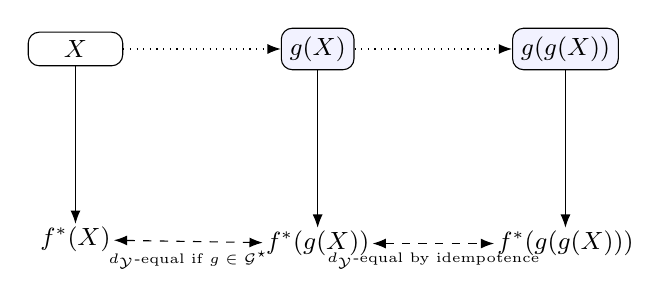
\begin{tikzpicture}[node distance=2cm]
\node[doc] (X) {$X$};
\node[sum, right=of X] (gX) {$g(X)$};
\node[sum, right=of gX] (ggX) {$g(g(X))$};

\node[op, below=of X] (fX) {$\fstar(X)$};
\node[op, below=of gX] (fgX) {$\fstar(g(X))$};
\node[op, below=of ggX] (fggX) {$\fstar(g(g(X)))$};

\draw[->, dotted] (X) -- node[above] {} (gX);
\draw[->, dotted] (gX) -- node[above] {} (ggX);
\draw[->] (X) -- node[left] {} (fX);
\draw[->] (gX) -- node[left] {} (fgX);
\draw[->] (ggX) -- node[left] {} (fggX);

\draw[<->, dashed] (fX) -- node[below] {\tiny $\metric$-equal if $g \in \Gstar$} (fgX);
\draw[<->, dashed] (fgX) -- node[below] {\tiny $\metric$-equal by idempotence} (fggX);
\end{tikzpicture}
\caption{Oracle-preserving normal form: one summarization preserves the task-relevant information, and re-summarizing an already-summarized text leaves it unchanged.}
\label{fig:gstar}
\end{figure}

\subsection{Document Decomposition}

When documents $x\in X$ exceed the length of LLM context windows, we cannot directly compute $g(x)$ without losing information (for example, by dropping all content in $x$ that exceeds the context window). Instead, we split documents into partitions, summarize partitions, and then summaries collections of summaries, until $x$ can be summarized by a single summary $g(x)$. We refer to this general procedure as \textit{hierarchical summarization}. 

Fix a partition of a document $x$ into contiguous blocks $(b_1,\ldots,b_k)$ with $b_1\concat\cdots\concat b_k=x$. A \emph{reduction tree} $T$ is any full binary tree whose leaves, read left-to-right, are $(b_1,\ldots,b_k)$. Given $g$, define the hierarchical reduction recursively by
\[
\reduceg(T)\;=\;
\begin{cases}
g(b_i), & \text{if $T$ is the leaf }b_i,\\[3pt]
g\!\big(\reduceg(T_L)\concat \reduceg(T_R)\big), & \text{if $T$ has left/right subtrees }T_L,T_R.
\end{cases}
\]
A second ``round'' applies $g$ again to the result, and so on:
\[
Z^{(1)}(x)\;:=\;\reduceg(T),\qquad
Z^{(R+ 1)}(x)\;:=\;g\!\big(Z^{(R)}(x)\big)\quad\text{for }R\ge1.
\]
This notation captures both one-pass reductions and deployments that apply additional normalization passes.

While notationally simple, this left-to-right structure is more restrictive than analysts may desire in practice. Many pipelines first reduce within larger contiguous units (e.g., articles within an issue) and then merge those summaries. Formally, we coarsen the leaves into contiguous folds $F_1,\ldots,F_J$, reduce each $F_j$ with an arbitrary within-fold tree $T_j$ to obtain $S_j=\reduceg(T_j)$, then reduce the sequence $(S_1,\ldots,S_J)$ along any binary tree $\widehat T$. The resulting \emph{fold-of-folds} output is $Z_{\mathrm{fold}}(x):=\reduceg(\widehat T)$. When compatibility laws (discussed below) apply, our guarantees apply to every (reasonable) choice of $(T_1,\ldots,T_J,\widehat T)$.

Figure \ref{fig:hierarchical_summarization} graphically depicts a common hierarchical summarization procedure. 



\begin{figure}[t]
\centering
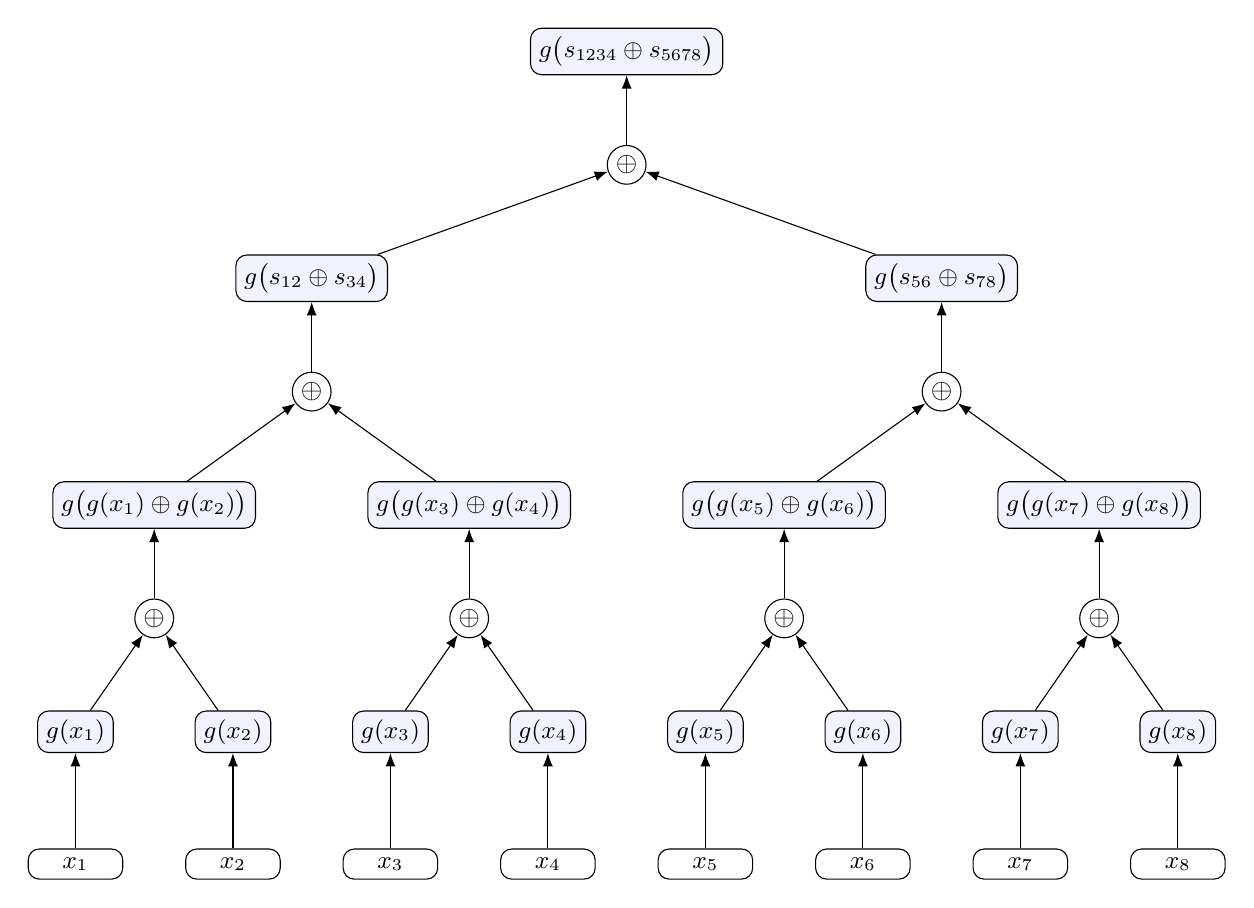
\begin{tikzpicture}[x=1.0cm, y=1.2cm]  % tighten x to keep the full tree within page width
  % Optional: a style to highlight nodes we sample for oracle checks later.
  % Usage: replace 'doc' or 'sum' with 'doc,selected' or 'sum,selected' on any node.
  \tikzset{selected/.style={fill=yellow!30, draw=orange!80!black, very thick}}

  %  --  Bottom row: documents x_1,...,x_8 and their first summaries g(x_i)
  \foreach \i [evaluate=\i as \xx using 2*(\i-1)] in {1,...,8}{
    \node[doc] (x\i) at (\xx,0) {$x_{\i}$};                 % e.g., add [selected] here to highlight a leaf
    \node[sum] (g\i) at (\xx,1.4) {$g(x_{\i})$};
    \draw[->] (x\i) -- (g\i); % upward "summarize"
  }

  %  --  Level 1 merges: (1,2), (3,4), (5,6), (7,8)
  \foreach \a/\b in {1/2,3/4,5/6,7/8}{
    \node[plus] (p\a\b) at ($ (g\a)!0.5!(g\b) + (0,1.2) $) {$\concat$};
    \node[sum]  (s\a\b) at ($ (p\a\b) + (0,1.2) $) {$g\big(g(x_{\a}) \concat g(x_{\b})\big)$};
    \draw[->] (g\a) -- (p\a\b);
    \draw[->] (g\b) -- (p\a\b);
    \draw[->] (p\a\b) -- (s\a\b);
  }

  %  --  Level 2 merges: (12,34) and (56,78)
  \foreach \L/\R in {12/34,56/78}{
    \node[plus] (p\L\R) at ($ (s\L)!0.5!(s\R) + (0,1.2) $) {$\concat$};
    \node[sum]  (s\L\R) at ($ (p\L\R) + (0,1.2) $) {$g\big(s_{\L} \concat s_{\R}\big)$};
    \draw[->] (s\L) -- (p\L\R);
    \draw[->] (s\R) -- (p\L\R);
    \draw[->] (p\L\R) -- (s\L\R);
  }

  %  --  Top merge: (1234, 5678)
  \node[plus] (pall) at ($ (s1234)!0.5!(s5678) + (0,1.2) $) {$\concat$};
  \node[sum]  (sall) at ($ (pall) + (0,1.2) $) {$g\big(s_{1234} \concat s_{5678}\big)$};
  \draw[->] (s1234) -- (pall);
  \draw[->] (s5678) -- (pall);
  \draw[->] (pall) -- (sall);

  % If we later want a visible legend without cluttering edges:
  % \node[op, anchor=west] at ($(x1.west)+(-0.5,0)$) {\emph{All upward arrows apply $g$; circles mark concatenation.}};
\end{tikzpicture}
\caption{Hierarchical summarization as a binary tree. Bottom documents $x_i$ are summarized by $g$; summaries are concatenated and re-summarized up the tree until a single top summary remains. No oracle $\fstar$ evaluations are required except (optionally) as accuracy checks.}
\label{fig:hierarchical_summarization}
\end{figure}

\subsection{Local Compatibility laws}\label{sec:compatibility}

When a document $x=b_1\concat\cdots\concat b_k$ is processed hierarchically, we want conditions that are both \emph{local} (they speak only about the leaves and internal pairs actually realized by the scheduler) and \emph{auditable} (they can be checked on held‑out trees) and that are sufficient to preserve $\fstar(x)$ under one pass and under additional normalization rounds. Throughout, expectations with the subscript $g$ average only over the internal randomness of $g$, conditional on the argument(s) being summarized and on the realized partition and merge schedule; population expectations $\E[\cdot]$ further average over $X\sim\Law$ and any external randomness in the partition and schedule, where $\Law$ represents the underling data-generating process of $X$.

\paragraph{Realized strings, reductions, and edges.}
Fix a full binary reduction tree $T$ whose leaves, read left to right, are the contiguous blocks $(b_1,\ldots,b_k)$ of $x$. For any node $u$ in $T$, the \emph{realized string at $u$} is defined recursively by
\[
S(u)=
\begin{cases}
b_i, & \text{if $u$ is the $i$th leaf},\\[2pt]
S(u_L)\concat S(u_R), & \text{if $u$ is internal with children $u_L,u_R$}.
\end{cases}
\]
Given a (possibly stochastic) summarizer $g$, the \emph{one‑pass hierarchical reduction at $u$} is
\[
\reduceg(u)=
\begin{cases}
g\!\big(S(u)\big), & \text{if $u$ is a leaf},\\[2pt]
g\!\Big(\reduceg(u_L)\ \concat\ \reduceg(u_R)\Big), & \text{if $u$ is internal}.
\end{cases}
\]
We write $\mathrm{root}(T)$ for the root node and set $Z^{(1)}(x):=\reduceg(\mathrm{root}(T))$. For $R\ge 2$, further \emph{normalization rounds} are defined by $Z^{(R)}(x):=g\!\big(Z^{(R-1)}(x)\big)$. The \emph{realized internal edges} of $T$ are the ordered pairs $(v,w)=\big(S(u_L),S(u_R)\big)$ at each internal node $u$.

When we need to emphasize the scope of internal randomness, we write $\Eg^{\downarrow u}[\cdot]$ for the expectation over \emph{all} coin flips of $g$ used to compute $\reduceg(u_L)$, $\reduceg(u_R)$, and the subsequent parent call at $u$, conditional on the realized strings $S(u_L)$ and $S(u_R)$ and on the realized partition (schedule).

\begin{figure}
    \centering
    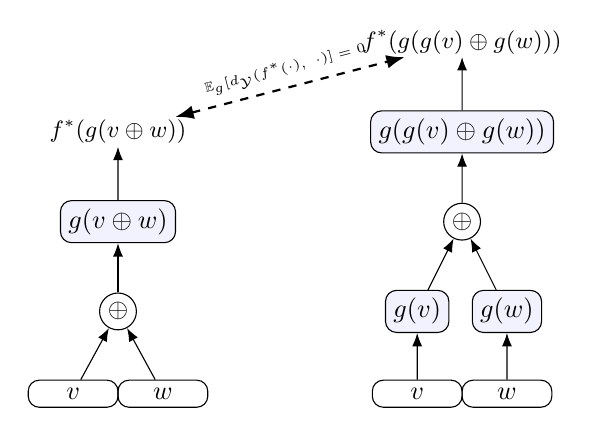
\begin{tikzpicture}[node distance=8.5mm and 10.5mm,scale=0.95, every node/.style={transform shape}]
% Route 1
\node[doc] (a1) at (0,0) {$v$};
\node[doc] (b1) at (1.2,0) {$w$};
\node[plus] (plus1) at (0.6,1.1) {$\concat$};
\node[sum] (gab) at (0.6,2.3) {$g(v \concat w)$};
\node[op] (f1) at (0.6,3.5) {$\fstar(g(v \concat w))$};
\draw[->] (a1) -- (plus1);
\draw[->] (b1) -- (plus1);
\draw[->] (plus1) -- (gab);
\draw[->] (gab) -- (f1);

% Route 2
\node[doc] (a2) at (4.6,0) {$v$};
\node[doc] (b2) at (5.8,0) {$w$};
\node[sum] (ga) at (4.6,1.1) {$g(v)$};
\node[sum] (gb) at (5.8,1.1) {$g(w)$};
\node[plus] (plus2) at (5.2,2.3) {$\concat$};
\node[sum] (ggab) at (5.2,3.5) {$g(g(v) \concat g(w))$};
\node[op] (f2) at (5.2,4.7) {$\fstar(g(g(v) \concat g(w)))$};
\draw[->] (a2) -- (ga);
\draw[->] (b2) -- (gb);
\draw[->] (ga) -- (plus2);
\draw[->] (gb) -- (plus2);
\draw[->] (plus2) -- (ggab);
\draw[->] (ggab) -- (f2);

\draw[<->, dashed, thick] (f1) -- node[above, sloped] {\tiny $\Eg[\metric(\fstar(\cdot),\ \cdot)]=0$} (f2);
\end{tikzpicture}
    \caption{Edge-wise compatibility at a realized merge. 
At an internal node with children $(v,w)$, there are two admissible routes to the parent's oracle: 
\emph{(left)} concatenate the underlying strings and summarize once, then apply $\fstar$; 
\emph{(right)} summarize each child, concatenate the summaries, and summarize once more, then apply $\fstar$. 
Parentwise compatibility \ref{eq:leaf_compatibility} requires these two routes to agree in expectation given the realized subtree, i.e., 
$\Eg^{\downarrow u}\big[\,\metric(\fstar(g(\reduceg(u_L)\concat \reduceg(u_R))),\,\fstar(S(u)) )\,\big]=0$. 
For audits, the edge-wise probe compares the two routes directly at the realized edge $(v,w)$ by checking 
$\metric\!\big(\fstar(v\concat w),\,\fstar(g(g(v)\concat g(w)))\big)=0$ (Equation~\ref{eq:edgewise_equivalence}). When both children $v$ and $w$ are on‑range of $g$, the parent’s oracle depends only on the children’s oracle values, and \ref{eq:leaf_compatibility} and \ref{eq:edgewise_equivalence} coincide.}
    \label{fig:local_compatibility}
\end{figure}


Figure~\ref{fig:local_compatibility} displays the two routes that meet at a single realized internal edge $(v,w)$ in the reduction tree. The left route concatenates the underlying child strings, summarizes once, and then evaluates the oracle; the right route summarizes each child, concatenates the summaries, and summarizes once more before evaluating the oracle. Our compatibility requirement is deliberately local: these two routes must agree at the oracle in expectation with respect to the summarizer's internal randomness, conditional on the realized subtree. This edge‑level picture is the operational unit we can actually audit in deployed hierarchies.

\paragraph{Three local laws.}
All three laws are stated on the \emph{realized} leaves and internal pairs of $T$. If $g$ is deterministic, expectations can be dropped and equalities are pointwise.


% --- Local laws with custom tags L1--L3 ---
% Leaf sufficiency in expectation

Our first local law is called \textit{Leaf Sufficiency (in expectation)}:

\begin{equation}\tag{L1}\label{eq:leaf_sufficiency}
\Eg\!\big[\,\metric\big(\fstar(g(b)),\,\fstar(b)\big)\,\big]\;=\;0
\quad\text{for every realized leaf }b.
\end{equation}

Next, we have \textit{Parentwise Compatibility}:

% Parentwise compatibility
\begin{equation}\tag{L2}\label{eq:leaf_compatibility}
\Eg^{\downarrow u}\!\Big[
  \metric\Big(\,\fstar\!\big(g\!\big(\reduceg(u_L)\concat \reduceg(u_R)\big)\big),\
                 \fstar\!\big(S(u)\big)\,\Big)\Big]\;=\;0
\quad\text{for every realized internal node }u.
\end{equation}

In words: along the particular subtree beneath $u$, if we reduce the children exactly as the hierarchy does and then summarize their concatenation at the parent, the expected oracle at the parent equals the ground‑truth oracle of the underlying concatenation.


Finally, we have \textit{On-Range Idempotence}:

% On-range stability (re-summarization idempotence)
\begin{equation}\tag{L3}\label{eq:leaf_idempotence}
\Eg\!\big[\,\metric\big(\fstar(g(Z)),\,\fstar(Z)\big)\,\big|\,Z\big]\;=\;0
\quad\text{for every $Z$ supported on the range of $g$}.
\end{equation}

Equivalently, once a string lies on the range of $g$, re‑applying $g$ does not change its oracle in expectation.


These conditions are strictly local: they quantify only over the leaves and internal nodes the scheduler \emph{actually} realized on $x$; no claims are made about unobserved pairs in $\Strings\times\Strings$, and no global associativity or commutativity is assumed.

\begin{remark}[Edge-wise compatibility]\label{rem:edgewise_compatibility}
Some audits might prefer to check a more granular \emph{edge‑wise} two‑route identity at internal edges $(v,w)=\big(S(u_L),S(u_R)\big)$:
\begin{equation}\tag{E1}\label{eq:edgewise_equivalence}
% \fstar(v\concat w)\;=\;\Eg\!\left[\,\fstar\!\Big(g\big(g(v)\ \concat\ g(w)\big)\Big)\,\right].
\metric\big(\fstar(v\concat w),\,\fstar(g(g(v)\concat g(w)))\big)=0
\end{equation}
Eq.\,\eqref{eq:edgewise_equivalence} compares ``summarize–concatenate–re‑summarize'' to the direct oracle on the underlying concatenation \emph{for that edge}. It is easy to audit and can meaningfully complement \eqref{eq:leaf_compatibility}. In general neither \eqref{eq:edgewise_equivalence} nor \eqref{eq:leaf_sufficiency} and \eqref{eq:leaf_compatibility} implies the other without additional structure (unless of course both children are leaves, in which case \eqref{eq:leaf_sufficiency} reduces exactly to \eqref{eq:edgewise_equivalence}); under further assumptions (e.g., when the parent call, given on‑range inputs, depends only on the children's oracle values) the two can be linked. Our invariance results below require only \eqref{eq:leaf_sufficiency}, \eqref{eq:leaf_compatibility}, and \eqref{eq:leaf_idempotence}.
\end{remark}

\paragraph{What the local laws buy.}
The next theorem is the basic preservation result for a single hierarchical pass; it uses only leaf sufficiency and parentwise compatibility.


\begin{theorem}[One‑pass preservation under leaf sufficiency and parentwise compatibility]\label{thm:one-pass}
Fix $x=b_1\concat \cdots\concat b_k$ and a full binary tree $T$ on these leaves.
If \ref{eq:leaf_sufficiency} holds on every realized leaf and \ref{eq:leaf_compatibility} holds at every realized internal node, then
\[
\Eg\!\left[\,\metric\!\Big(\fstar\big(\reduceg(\mathrm{root}(T))\big),\ \fstar(x)\Big)\,\right]\;=\;0.
\]
\end{theorem}


\begin{proof}
Proceed by structural induction on nodes, conditioning throughout on the realized strings $\{S(u)\}$. For a leaf $u=b$ we have $\reduceg(u)=g(b)$ and $\Eg[\fstar(\reduceg(u))]=\fstar(b)$ by \eqref{eq:leaf_sufficiency}. For an internal node $u$ with children $u_L,u_R$, by definition
\[
\reduceg(u)=g\!\left(\reduceg(u_L)\ \concat\ \reduceg(u_R)\right).
\]
Taking $\fstar$ and $\Eg^{\downarrow u}$ and applying \eqref{eq:leaf_compatibility} yields
$\Eg^{\downarrow u}\!\left[\fstar(\reduceg(u))\right]=\fstar\!\big(S(u)\big)$.
Inducting up to the root gives the claim with $S(\mathrm{root}(T))=x$.
\end{proof}

Because the proof only used local equalities at realized internal nodes, the expected oracle is invariant to the merge schedule.

\begin{corollary}[Schedule invariance: chain vs.\ batch]\label{cor:schedule}
Under the hypotheses of Theorem~\ref{thm:one-pass}, the equality
$\Eg\big[\metric\big(\fstar(\reduceg(\mathrm{root}(T)),\fstar(x)\big)\big] = 0$
holds for \emph{every} full binary tree $T$ on the fixed leaf partition $(b_1,\ldots,b_k)$ whose nodes satisfy \eqref{eq:leaf_sufficiency} and \eqref{eq:leaf_compatibility}. In particular, balanced trees and daisy‑chain schedules agree in expected oracle value.
\end{corollary}

The same argument applies to two‑level pipelines that first reduce within larger contiguous units and then reduce the sequence of fold‑summaries under any binary tree.

\begin{corollary}[Fold‑of‑folds invariance]\label{cor:folds}
Let $(F_1,\ldots,F_J)$ be a contiguous coarsening of the leaves. Reduce each fold $F_j$ by an arbitrary within‑fold tree $T_j$ to obtain $S_j:=\reduceg(T_j)$, then reduce $(S_1,\ldots,S_J)$ by any over‑fold tree $\widehat T$. If \eqref{eq:leaf_sufficiency} holds on all realized leaves across both levels and \eqref{eq:leaf_compatibility} holds at every realized internal node, then
% \[
% \Eg\!\big[\ \fstar\big(\reduceg(\widehat T)\big)\ \big]\;=\;\fstar(x).
% \]
\[
\Eg\!\big[\ \metric\big(\fstar\big(\reduceg(\widehat T)\big),\ \fstar(x)\big)\big] = 0.
\]
\end{corollary}

Finally, the stability law guarantees that extra normalization rounds are inert at the oracle.

\begin{theorem}[Multi‑round preservation by on‑range stability]\label{thm:multi-round}
Assume the hypotheses of Theorem~\ref{thm:one-pass}, so that
\[
\Eg\Big[\metric\big(\fstar(Z^{(1)}(x)),\,\fstar(x)\big)\Big]=0.
\]
If, in addition, \ref{eq:leaf_idempotence} holds, then for every $R\ge 1$,
\[
\Eg\Big[\metric\big(\fstar(Z^{(R)}(x)),\,\fstar(x)\big)\Big]=0,
\qquad
Z^{(1)}(x):=\reduceg(\mathrm{root}(T)),\ \ Z^{(R+1)}(x):=g\!\big(Z^{(R)}(x)\big).
\]
\end{theorem}


\paragraph{Interpretation and auditability.}
The three laws isolate exactly what deployed systems expose. Leaf sufficiency \eqref{eq:leaf_sufficiency} asks that a single call to $g$ preserve the oracle on the blocks we actually feed it. Parentwise compatibility \eqref{eq:leaf_compatibility} demands that, at each realized internal node, the two routes—reduce the children as scheduled and then summarize their concatenation, versus apply the oracle to the underlying concatenation—match in expectation. Stability \eqref{eq:leaf_idempotence} certifies that further normalization passes are inert at the oracle. All statements tolerate stochastic $g$ and arbitrary parenthesization; no global algebra is assumed. For audits that prefer edge‑level probes, the optional law \eqref{eq:edgewise_equivalence} compares the two routes at a single edge; it can be sampled and tested directly and, in many applications, serves as a convenient stress test alongside \eqref{eq:leaf_compatibility}. In Section \ref{sec:dpo}, we discuss how to bound accumulated error when sufficiency is only approximately, and not exactly, achievable. 




\subsection{What the local laws buy us}\label{sec:what-local-buys}

The point of the local laws is operational control where the system actually runs. The three laws---leaf sufficiency \eqref{eq:leaf_sufficiency}, parentwise compatibility \eqref{eq:leaf_compatibility} (and the auditable edge form \eqref{eq:edgewise_equivalence}), and on-range stability \eqref{eq:leaf_idempotence}---deliver four concrete consequences.

\begin{enumerate}[wide,label=\textbf{(\alph*)},leftmargin=*]

\item \textbf{Processing invariance without global algebra.} 
By Theorem~\ref{thm:one-pass}, a single hierarchical pass preserves the oracle in expectation for \emph{any} full binary tree on a fixed partition. Corollary~\ref{cor:schedule} then yields schedule invariance (balanced tree vs.\ daisy chain), and Corollary~\ref{cor:folds} yields fold-of-folds invariance. No associativity or commutativity of a hidden merge operator is assumed; we only require equalities \emph{at the internal merges that actually occurred}.

\item \textbf{Auditability at deployment.}
Every constraint is stated on realized leaves and realized internal pairs, which is exactly what the pipeline exposes and what we can sample on held-out runs. Section~\ref{sec:audit} composes the resulting empirical rates into an end-to-end bound.

\item \textbf{Tolerance to stochasticity and reprocessing.}
The equalities are imposed in expectation with respect to $g$'s internal randomness, so stochastic summarizers are admissible. Theorem~\ref{thm:multi-round} shows additional ``normalization'' rounds are inert in expectation if and only if  $g$ is on-range idempotent at the oracle, i.e.\ \eqref{eq:leaf_idempotence} holds.

\item \textbf{Separation of task semantics from string details.}
What is preserved is $\fstar$, not any particular concrete summary string. This permits supervision to be ``transported'' through the hierarchy (Lemma~\ref{lem:blackwell-transport}), and later allows preference training (e.g., DPO) on summaries to attain the same population optimum as training on full documents under exact preservation; under approximate preservation, the population gap is controlled quantitatively (Theorem~\ref{thm:dpo-gap}).

\end{enumerate}

\section{From local laws to learnable bottlenecks: existence, score transport, and preparation for DPO}
\label{sec:exist-learn-transport}

This section consolidates what the local laws buy us, strengthens the score‑transport argument to a Blackwell‑style sufficiency statement, and records two existence results phrased in the \emph{metric} language used throughout. The guiding principle is that downstream supervision cares only about $\fstar(\cdot)$ measured in the task metric $\metric$; string‑level details should matter only insofar as they change $\metric(\fstar(\cdot),\cdot)$.

\paragraph{What the local laws imply (recap).}
Leaf sufficiency \eqref{eq:leaf_sufficiency} and parentwise compatibility \eqref{eq:leaf_compatibility} imply one–pass preservation of the oracle in expectation for any full binary merge tree by Theorem~\ref{thm:one-pass}. The conclusion is \emph{schedule‑invariant} (balanced tree vs.\ daisy chain) by Corollary~\ref{cor:schedule}, and extends to fold‑of‑folds schedules (Corollary~\ref{cor:folds}). On‑range stability \eqref{eq:leaf_idempotence} makes further normalization rounds inert at the oracle (Theorem~\ref{thm:multi-round}). These statements are deliberately local and auditable: they speak only about the leaves and internal pairs the realized scheduler actually executed.


\subsection{Score transport via Blackwell sufficiency}
\label{sec:transport}

Recall Assumption~\ref{ass:CF}: there exists a measurable $\bar Q:\Y\times\A\to\mathbb{R}$ with
$\E[\sstar(X,a)\mid X]=\bar Q(\fstar(X),a)$ for all $a\in\A$.
The right notion of ``no information loss'' for learning is that the summary exposes at least as much \emph{oracle information} as the document for the purpose of predicting the score.



\begin{lemma}[Blackwell/Doob–Dynkin score transport]
\label{lem:blackwell-transport}
Assume Assumption~\ref{ass:CF}. Let $Z$ be any representation with $\sigma(\fstar(X))\subseteq\sigma(Z)$.
Then for every $a\in\A$,
\[
\E\!\big[\sstar(X,a)\big]\ =\ \E\!\big[\sstar_Z(Z,a)\big]\ =\ \E\!\big[\bar Q(\fstar(X),a)\big].
\]
Moreover, for any bounded linear functional $\Lambda$ on the Banach space $(\mathcal{B}(\A),\|\cdot\|_\infty)$ of bounded real functions on $\A$,
\[
\E\!\big[\Lambda\big(\sstar(X,\cdot)\big)\big]
\ =\
\E\!\big[\Lambda\big(\sstar_Z(Z,\cdot)\big)\big]
\ =\
\E\!\big[\Lambda\big(\bar Q(\fstar(X),\cdot)\big)\big].
\]
\end{lemma}


In particular, when the local laws hold \emph{exactly} along the realized tree so that $\fstar(Z^{(R)}(X))=\fstar(X)$ almost surely (Theorems~\ref{thm:one-pass} and \ref{thm:multi-round}), we may take $Z=Z^{(R)}(X)$ and conclude that all linearly aggregated supervision (proper scoring risks, linear utilities, etc.) are unchanged by hierarchical processing. For nonlinear objectives (e.g., logistic transforms in preference learning), equality need not hold. In that case we control the discrepancy by the deployment‑level \emph{oracle distortion}
\[
\Delta_R\ :=\ \E\!\big[\,\metric\!\big(\fstar(Z^{(R)}(X)),\,\fstar(X)\big)\,\big],
\]
which is bounded additively by \emph{operation‑level} distortions in Appendix~\ref{sec:audit}.


\subsection{Parentwise vs.\ edgewise compatibility}\label{sec:parent-vs-edge}

Parentwise compatibility \eqref{eq:leaf_compatibility} is what is used in the induction proof of Theorem~\ref{thm:one-pass}. Alternatively, researchers might prefer the following edge‑wise, two‑route audit:

\begin{equation}\label{eq:edgewise-metric}\tag{Edge}
\metric\!\Big(\fstar(v\concat w),\ \fstar\big(g(g(v)\concat g(w))\big)\Big)=0
\qquad\text{for a realized internal edge }(v,w).
\end{equation}

When both child inputs at a parent are already on the range of $g$ (as they are in the realized reduction), \eqref{eq:edgewise-metric} and \eqref{eq:leaf_compatibility} can be directly linked under Assumption~\ref{ass:app3} and the discussion in Section~\ref{sec:global}. If $u_L,u_R$ are leaves, \eqref{eq:leaf_compatibility} reduces exactly to \eqref{eq:edgewise-metric}. Thus the proofs need \eqref{eq:leaf_compatibility}; audits may test either \eqref{eq:leaf_compatibility} or \eqref{eq:edgewise-metric} on the edges the scheduler actually realizes.

\subsection{Stability is substantive}
\label{sec:stability-caution}
On‑range stability \eqref{eq:leaf_idempotence} is not a cosmetic clean‑up. Without it, ``normalize again'' can flip $\fstar$ even if \eqref{eq:leaf_sufficiency}–\eqref{eq:leaf_compatibility} hold. A minimal counterexample is a summarizer that maps every positive leaf to a special token $\mathsf{POS}$ but, when prompted with $\mathsf{POS}$, returns $\mathsf{NEG}$. Leaf sufficiency holds, parentwise equalities can pass, yet a second pass flips the oracle at the root. This is why we audit on‑range behavior at sampled roots and recommend prompts that make $g$ act like a canonicalization map on its own range.


\subsection{Oracle‑preserving summarizers}
\label{sec:existence}


We now connect oracle‑preserving hierarchies to Direct Preference Optimization (DPO). Preference data consist of triples $(x,a_w,a_\ell)$ with a binary label indicating the winner. Under the standard Bradley–Terry–Luce factorization, the conditional preference probability depends on $x$ only through $\fstar(x)$:
\begin{equation}\label{eq:BT-oracle}
\Prob\{a_w\succ a_\ell\mid X=x\}\;=\;\sigma\!\Big(\beta\,[R_{\fstar(x)}(a_w)-R_{\fstar(x)}(a_\ell)]\Big),
\qquad\sigma(t)=\frac{1}{1+ e^{-t}},
\end{equation}
for some per‑oracle reward family $\{R_y:\A\to\R\}_{y\in\Y}$ and scale $\beta>0$.
DPO reparameterizes the reward through the policy $\pi$ relative to a reference $\pi_{\mathrm{ref}}$ and minimizes
\begin{equation}\label{eq:dpo-loss}
\mathcal{L}_{\mathrm{DPO}}(\pi;\pi_{\mathrm{ref}})
=-\,\E\Bigg[\log \sigma\!\Big(\beta\Big[
\log\frac{\pi(a_w\mid X)}{\pi_{\mathrm{ref}}(a_w\mid X)}-\log\frac{\pi(a_\ell\mid X)}{\pi_{\mathrm{ref}}(a_\ell\mid X)}
\Big]\Big)\Bigg].
\end{equation}

Two existence notions matter: set‑theoretic (\emph{some} $g$ exists) and operational (a \emph{short} $g$ exists that fits a budget). We state both in terms of the task metric.

\begin{proposition}[Canonical representative map in metric form]
\label{prop:canonical}
Because $\Strings$ is countable, define $x\sim x'$ iff $\metric(\fstar(x),\fstar(x'))=0$. Fix a total order on $\Strings$ and let $c:\Y\to\Strings$ send $y$ to the least $x$ with $\metric(\fstar(x),y)=0$. Then
\[
g_{\mathrm{can}}(x):=c\big(\fstar(x)\big)
\quad\text{satisfies}\quad
\metric\!\big(\fstar(g_{\mathrm{can}}(x)),\,\fstar(x)\big)=0\ \ \text{for all }x,
\]
and $g_{\mathrm{can}}$ is idempotent on its range. Hence $g_{\mathrm{can}}\in\Gstar$ in the sense of Definition~\ref{def:exact-suff-stable}.
\end{proposition}

\begin{proposition}[Compact encodings]
\label{prop:encoding}
If there exists an injective encoder $\mathrm{enc}:\Y\to\Strings$ of uniformly bounded length such that
$\metric(\fstar(\mathrm{enc}(y)),y)=0$ for all $y\in\Y$, then
\[
g_{\mathrm{enc}}(x):=\mathrm{enc}(\fstar(x))
\quad\text{obeys}\quad
\metric\!\big(\fstar(g_{\mathrm{enc}}(x)),\,\fstar(x)\big)=0
\]
and is idempotent on its range. Thus $g_{\mathrm{enc}}\in\Gstar$ and returns short strings.
\end{proposition}

Proposition~\ref{prop:canonical} certifies internal consistency: exact, idempotent, oracle‑preserving normal forms always exist; Proposition~\ref{prop:encoding} records the operational version used in practice (the summary \emph{is} a compact encoding of the oracle).


\subsection{How to learn sufficient summaries in practice}
\label{sec:learning-g}

There are two concrete routes tightly aligned with the laws. In a supervised route, parameterize $g_\phi$ and a decoder $h_\psi$ and minimize a proper $\Y$‑loss on $h_\psi(g_\phi(x))$ while regularizing the three local laws on realized leaves and internal nodes:
\[
\metric\!\big(\fstar(b),h_\psi(g_\phi(b))\big)\;\concat \;
\metric\!\big(h_\psi(g_\phi(v\concat w)),h_\psi(g_\phi(g_\phi(v)\concat g_\phi(w)))\big)\;\concat \;
\metric\!\big(h_\psi(g_\phi(z)),h_\psi(z)\big).
\]
In a preference route, optimize a preference objective \emph{on summaries} with the same regularizers to keep $g_\phi$ near $\Gstar$. In both cases the audit in Appendix~\ref{sec:audit} turns observed operation‑level distortions into a deployment‑level bound $\Delta_R$ that propagates to task and DPO gaps.



\section{Conclusion and Outlook}\label{sec:conclusion}

We recast long‑document processing as an \emph{oracle‑preserving} reduction problem on the free monoid $(\Strings,\concat,\varnothing)$ with a task oracle $\fstar:\Strings\to Y$ and metric $\metric$ on $Y$. The focus is deliberately local. Three edge‑level laws—leaf sufficiency \ref{eq:leaf_sufficiency}, parentwise compatibility \ref{eq:leaf_compatibility}, and on‑range stability \ref{eq:leaf_idempotence}—are imposed only on the leaves and internal pairs the realized scheduler actually processes. This austerity is not cosmetic: it is exactly what a deployed hierarchy exposes and can be audited.

The guarantees follow directly from these local laws. Under \ref{eq:leaf_sufficiency}–\ref{eq:leaf_compatibility}, a single hierarchical pass preserves the oracle in expectation for any partition and any full binary merge tree $T$ on that partition. In particular, if $Z^{(1)}(x):=\reduceg(\mathrm{root}(T))$ is the one‑pass reduction of a document $x=b_1\concat \cdots\concat b_k$, then $\metric\!\big(\fstar(Z^{(1)}(x)),\fstar(x)\big)$ has mean zero, and the expected oracle is \emph{invariant} to parenthesization (balanced batch trees and daisy‑chains agree), including the usual ``fold‑of‑folds'' schedules. With \ref{eq:leaf_idempotence} as well, further normalization rounds $Z^{(R+ 1)}(x):=g(Z^{(R)}(x))$ are inert at the oracle in expectation, so repeated re‑summarization does not drift the task value.

These processing guarantees transport to learning under a classic sufficiency assumption. When supervision factorizes through the oracle—there is a measurable $\bar Q$ with $\E[S^\star(X,a)\mid X]=\bar Q(\fstar(X),a)$—preference training on oracle‑preserving summaries is information‑equivalent to training on full documents. In particular, for Direct Preference Optimization (DPO), if the hierarchy preserves $\fstar$ along the realized tree, the set of population minimizers is unchanged and the Bayes‑optimal KL‑regularized policy depends on inputs only through $\fstar(\cdot)$. When preservation holds only approximately, the population gap is controlled quantitatively by a single deployment‑level distortion
\[
\Delta_R\ :=\ \E\Big[\,\metric\!\big(\fstar(Z^{(R)}(X)),\,\fstar(X)\big)\Big],
\]
with explicit envelopes (e.g., Lipschitz policies or rewards) turning $\Delta_R$ into a numerical bound on the DPO loss difference.

A key practical contribution is an operational audit that matches how systems are built. The audit samples \emph{realized} leaves and internal nodes, measures the corresponding oracle distortions under \ref{eq:leaf_sufficiency} and \ref{eq:leaf_compatibility}, probes on‑range stability for any additional rounds, and composes these terms to certify $\Delta_R$ for the deployed partition and tree. Because the estimates are tied to the operations the hierarchy actually executed, the audit provides deployment‑specific error budgets that make visible the trade‑offs among block size, merge schedule, cost, and accuracy.

For text‑as‑data applications, the implications are concrete. Many designs collapse long, heterogeneous texts to structured signals—binary event indicators, actor–action–target–time–place tuples, or counts. Our results state precisely when such hierarchical preprocessing leaves the target intact and show how to certify that fact from the pipeline's own operations. The limits are equally clear. The strongest equivalences require that supervision really factor through $\fstar$; if annotators reward presentational features not encoded by the oracle, training on summaries can deviate even when the edge‑wise laws hold. And while a global algebraic variant connects to monoid congruences and mergeable sketches, none of the guarantees above depend on global associativity that the task semantics may not justify.

Methodologically, the blueprint is simple but demanding. Build hierarchies that pass the edge‑wise audit; train preference‑optimized policies on their outputs; and report certified error budgets alongside codebooks and models. The result is a pipeline whose guarantees align with the codebook, whose failures are interpretable, and whose outputs can be trusted to mean what the research design claims they mean.


\bibliographystyle{plainnat}
\bibliography{refs}


\appendix

\section{Notation Recap and Standing Assumptions}
\label{app:notation}

We work on the free monoid $(\Strings,\concat ,\varnothing)$ with concatenation $\concat $ and empty string $\varnothing$.
Documents are random $X\in \Strings$ from a population law $\rho$. A fixed ``oracle" $\fstar:\Strings\to Y$ maps any string to the task value (label/tuple/score). We fix a (pseudo)metric $\metric$ on $Y$ and measure distortion by $D(z\|x):=\metric\big(\fstar(z),\fstar(x)\big)$.

A (possibly stochastic) summarizer $g:\Strings\rightsquigarrow \Strings$ turns strings into strings; $\Eg[\cdot]$ averages over the \emph{internal} randomness of $g$, holding fixed its input; outer expectations $\E[\cdot]$ also average over $X\sim\rho$ and any randomness in partitioning/scheduling.

For hierarchical processing: partition $x=b_1\concat \cdots\concat b_k$ into contiguous blocks; fix any full binary tree $T$ with leaves $(b_1,\dots,b_k)$. Define the realized string at node $u$ by
\[
S(u)=
\begin{cases}
b_i,&u\text{ is the $i$th leaf},\\
S(u_L)\concat S(u_R),&u\text{ internal with children }u_L,u_R.
\end{cases}
\]
Define the one-pass reduction $\reduceg(u)$ recursively by
\[
\reduceg(u)=
\begin{cases}
g\!\left(S(u)\right),&u\text{ leaf},\\
g\!\left(\reduceg(u_L)\concat \reduceg(u_R)\right),&u\text{ internal}.
\end{cases}
\]
Write $Z^{(1)}(x):=\reduceg(\mathrm{root}(T))$ and $Z^{(R+ 1)}(x):=g\!\big(Z^{(R)}(x)\big)$ for $R\ge 1$.

\paragraph{Local laws (realized leaves and internal nodes).}
\begin{description}
  \item[\ref{eq:leaf_sufficiency} Leaf sufficiency in expectation.] For every realized leaf $b$, $\Eg\big[\metric\!\big(\fstar(g(b)), \fstar(b)\big)\big]=0$.
  \item[\ref{eq:leaf_compatibility} Parentwise compatibility.] For every realized internal node $u$,
  \[
  \E^{\downarrow u}_g\!\Big[\metric\!\Big(\fstar\!\big(g(\reduceg(u_L)\concat \reduceg(u_R))\big),\,\fstar\!\big(S(u)\big)\Big)\Big]=0,
  \]
  where $\E^{\downarrow u}_g$ averages over $g$-related randomness present below $u$ and at the parent call, conditional on the inputs $S(u_L),S(u_R)$.
  \item[\ref{eq:leaf_idempotence} On-range stability.] For any $Z$ supported on the range of $g$,
  $\Eg\!\big[\metric\!\big(\fstar(g(Z)),\fstar(Z)\big)\,\big|\,Z\big]=0$ a.s.
\end{description}

The edgewise identity for a realized internal edge $(v,w)=(S(u_L),S(u_R))$,
\[
\metric\!\Big(\fstar(v\concat w),\,\fstar\!\big(g\big(g(v)\concat g(w)\big)\big)\Big)=0,
\]
is a convenient audit probe and complements \ref{eq:leaf_compatibility}.

\section{Proofs of Propositions and Theorems in the Main Text}
\label{app:proofs-core}

Throughout this section we fix a document $x=b_1\concat\cdots\concat b_k\in\Strings$ together with a realized full binary reduction tree $T$ on the leaves $(b_1,\dots,b_k)$. For a node $u\in T$ we write $S(u)$ for the realized underlying string at $u$ and $\reduceg(u)$ for the one‑pass hierarchical reduction at $u$ as in Section~\ref{sec:compatibility}. Expectations with $\Eg^{\downarrow u}$ average \emph{only} over the internal randomness of $g$ used in the computation of $\reduceg(u_L)$, $\reduceg(u_R)$, and the parent call at $u$, conditional on the realized subtree below~$u$.

\medskip\noindent
We work entirely with the task pseudometric $\metric$ on $Y$; all conclusions are stated as equalities of the form $\Eg[\metric(\cdot,\cdot)]=0$ and never as expectations of $Y$–valued random variables.

\begin{lemma}[Nodewise preservation under the local laws]\label{lem:nodewise}
If the leaf sufficiency law \eqref{eq:leaf_sufficiency} holds on every realized leaf and the parentwise compatibility law \eqref{eq:leaf_compatibility} holds on every realized internal node, then for every node $u$ in $T$,
\[
\Eg^{\downarrow u}\!\Big[\ \metric\!\big(\fstar(\reduceg(u)),\ \fstar(S(u))\big)\ \Big]\;=\;0.
\]
\end{lemma}

\begin{proof}
Fix $u$. If $u$ is a leaf $b$, then $\reduceg(u)=g(b)$ and \eqref{eq:leaf_sufficiency} gives
$\Eg^{\downarrow u}\!\big[\metric(\fstar(\reduceg(u)),\fstar(S(u)))\big]
=\Eg\!\big[\metric(\fstar(g(b)),\fstar(b))\big]=0$.
If $u$ is internal with children $u_L,u_R$, then by definition
$\reduceg(u)=g\!\big(\reduceg(u_L)\concat \reduceg(u_R)\big)$
and parentwise compatibility \eqref{eq:leaf_compatibility} yields
$\Eg^{\downarrow u}\!\big[\metric(\fstar(\reduceg(u)),\fstar(S(u)))\big]=0$.
\end{proof}

\begin{theorem}[One‑pass preservation; Theorem~\ref{thm:one-pass}]\label{thm:one-pass-appendix}
Under the hypotheses of Lemma~\ref{lem:nodewise}, for the root node $r=\mathrm{root}(T)$,
\[
\Eg\!\Big[\ \metric\!\big(\fstar(\reduceg(r)),\ \fstar(x)\big)\ \Big]\;=\;0.
\]
\end{theorem}

\begin{proof}
Apply Lemma~\ref{lem:nodewise} with $u=r$. Since $\Eg^{\downarrow r}$ averages over precisely the coin flips used anywhere in the realized reduction of the entire tree (children and parent included), $\Eg^{\downarrow r}=\Eg$ for the fixed partition and schedule, and $S(r)=x$.
\end{proof}

\begin{corollary}[Schedule invariance; Corollary~\ref{cor:schedule}]
\label{cor:schedule-appendix}
The conclusion of Theorem~\ref{thm:one-pass-appendix} holds for every full binary tree $T$ on the fixed leaf partition $(b_1,\dots,b_k)$. In particular, for a given partition, balanced trees and daisy‑chain schedules agree in expected oracle value.
\end{corollary}

\begin{proof}
The proof of Lemma~\ref{lem:nodewise} and Theorem~\ref{thm:one-pass-appendix} uses only the local laws \eqref{eq:leaf_sufficiency}–\eqref{eq:leaf_compatibility} on the \emph{realized} leaves and internal nodes of the chosen $T$. Any other parenthesization realizes a (possibly different) set of internal nodes, but the same nodewise equalities apply to those nodes, yielding the same conclusion at the root.
\end{proof}


\begin{corollary}[Fold‑of‑folds invariance (Cor.~\ref{cor:folds})]\label{cor:folds2}
Let $(F_1,\ldots,F_J)$ be a contiguous coarsening of the leaves. For each $j$, fix an arbitrary full
binary within‑fold tree $T_j$ whose leaves, read left to right, concatenate to $F_j$. Let $\widehat T$ be any full
binary over‑fold tree whose leaves, read left to right, concatenate to $F_1+\cdots+F_J$. Form the
\emph{composite tree} $T_{\mathrm{comp}}$ by grafting $T_1,\ldots,T_J$ into $\widehat T$ at its $J$ leaves.

If \eqref{eq:leaf_sufficiency}holds on the realized leaves of $T_{\mathrm{comp}}$ and \eqref{eq:leaf_compatibility} holds at every realized internal node of $T_{\mathrm{comp}}$,
then
\[
\Eg\!\Big[\,\metric\!\big(\fstar(\reduceg(\mathrm{root}(T_{\mathrm{comp}}))),\ \fstar(x)\big)\,\Big]\;=\;0.
\]

In particular, the expected oracle at the root is invariant to the choice of the within‑fold parenthesizations and to the over‑fold parenthesization, provided the realized leaves and internal nodes of $T_{\mathrm{comp}}$ satisfy \eqref{eq:leaf_sufficiency}–\eqref{eq:leaf_compatibility}. Moreover, if \eqref{eq:leaf_idempotence} (on‑range stability) also holds, then for the usual two‑level “fold‑of‑folds” computation that first reduces each $F_j$ to $S_j:=\reduceg(T_j)$ and then reduces $(S_1,\ldots,S_J)$ along $\widehat T$, we have
\[
\Eg\!\Big[\,\metric\!\big(\fstar(\reduceg(\widehat T)),\ \fstar(x)\big)\,\Big]\;=\;0,
\]
because all additional $g$ calls at the leaves of $\widehat T$ are re‑applications of $g$ to on‑range strings and are inert at the oracle by \eqref{eq:leaf_idempotence}.
\end{corollary}

\begin{proof}
Apply Lemma~\ref{lem:nodewise} to the \emph{single} composite tree $T_{\mathrm{comp}}$. All its realized leaves and internal nodes are exactly the realized leaves and internal merges that occur across both levels, so the hypotheses \eqref{eq:leaf_sufficiency}–\eqref{eq:leaf_compatibility} on $T_{\mathrm{comp}}$ yield
\[
\Eg\!\Big[\,\metric\!\big(\fstar(\reduceg(\mathrm{root}(T_{\mathrm{comp}}))),\ \fstar(x)\big)\,\Big]\;=\;0.
\]
For the usual two‑level computation, view $\widehat T$ as a tree whose leaves are the strings $S_1,\ldots,S_J$. At those leaves, the algorithm applies $g$ once more to each $S_j$. Since each $S_j$ lies on the range of $g$, \eqref{eq:leaf_idempotence} implies $\metric\!\big(\fstar(g(S_j)),\fstar(S_j)\big)=0$ almost surely, so inserting these extra on‑range applications of $g$ leaves the oracle unchanged in expectation along $\widehat T$. Hence the displayed equality also holds with $\reduceg(\widehat T)$ in place of $\reduceg(\mathrm{root}(T_{\mathrm{comp}}))$.
\end{proof}


% \begin{corollary}[Fold‑of‑folds invariance; Corollary~\ref{cor:folds}]
% \label{cor:folds-appendix}
% Let $(F_1,\ldots,F_J)$ be a contiguous coarsening of the leaves. Reduce each fold $F_j$ by an arbitrary within‑fold tree $T_j$ to obtain $S_j:=\reduceg(T_j)$, then reduce $(S_1,\ldots,S_J)$ by any over‑fold tree $\widehat T$. If \eqref{eq:leaf_sufficiency} holds on all realized leaves across both levels and \eqref{eq:leaf_compatibility} holds at every realized internal node, then
% \[
% \Eg\!\big[\ \metric\big(\fstar\big(\reduceg(\widehat T)\big),\ \fstar(x)\big)\big]\;=\;0.
% \]
% \end{corollary}

% \begin{proof}
% Fix $j$ and condition on the $\sigma$‑field below $\mathrm{root}(T_j)$. Because \eqref{eq:leaf_sufficiency} holds on the realized leaves of $T_j$ and \eqref{eq:leaf_compatibility} holds at every realized internal node of $T_j$, Lemma~\ref{lem:nodewise} yields $\Eg^{\downarrow \mathrm{root}(T_j)}\!\big[\metric\big(\fstar(S_j),\fstar(F_j)\big)\big]=0$. Now view $\widehat T$ as a tree with leaves $(S_1,\ldots,S_J)$. Since \eqref{eq:leaf_sufficiency} also holds on these realized leaves and \eqref{eq:leaf_compatibility} holds at every realized internal node of $\widehat T$, a second application of Lemma~\ref{lem:nodewise} gives
% \[
% \Eg^{\downarrow \mathrm{root}(\widehat T)}\!\Big[\ \metric\!\big(\fstar\big(\reduceg(\widehat T)\big),\ \fstar(S_1\concat\cdots\concat S_J)\big)\ \Big]\;=\;0.
% \]
% By \eqref{eq:leaf_sufficiency}, replacing each $F_j$ by $S_j$ leaves the oracle target unchanged, so $\fstar(S_1\concat\cdots\concat S_J)=\fstar(F_1\concat\cdots\concat F_J)=\fstar(x)$. Taking expectations and using the tower property, the displayed conditional equality lifts to $\Eg\!\big[\metric\big(\fstar(\reduceg(\widehat T)),\fstar(x)\big)\big]=0$, as claimed.
% \end{proof}


\begin{theorem}[Multi‑round preservation; Theorem~\ref{thm:multi-round}]
\label{thm:multi-round-appendix}
Assume the hypotheses of Theorem~\ref{thm:one-pass-appendix} so that
\[
\Eg\!\Big[\ \metric\!\big(\fstar(Z^{(1)}(x)),\ \fstar(x)\big)\ \Big]=0,\qquad Z^{(1)}(x):=\reduceg(\mathrm{root}(T)).
\]
If, in addition, on‑range stability \eqref{eq:leaf_idempotence} holds, then for every $R\ge 1$,
\[
\Eg\!\Big[\ \metric\!\big(\fstar(Z^{(R)}(x)),\ \fstar(x)\big)\ \Big]\;=\;0,
\qquad Z^{(R+1)}(x):=g\!\big(Z^{(R)}(x)\big).
\]
\end{theorem}

\begin{proof}
For each $R\ge 1$ define the nonnegative quantity
\[
\Delta_R(x)\ :=\ \Eg\!\Big[\ \metric\!\big(\fstar(Z^{(R)}(x)),\ \fstar(x)\big)\ \Big].
\]
By Theorem~\ref{thm:one-pass-appendix}, $\Delta_1(x)=0$. Since $Z^{(R)}(x)$ is supported on the range of $g$ for all $R\ge 1$, on‑range stability \eqref{eq:leaf_idempotence} and the law of iterated expectations give
\[
\Eg\!\Big[\ \metric\!\big(\fstar(g(Z^{(R)}(x))),\ \fstar(Z^{(R)}(x))\big)\ \Big]=0.
\]
The triangle inequality therefore yields
\[
\Delta_{R+1}(x)\ =\ \Eg\!\Big[\ \metric\!\big(\fstar(Z^{(R+1)}(x)),\ \fstar(x)\big)\ \Big]
\ \le\
\underbrace{\Eg\!\Big[\ \metric\!\big(\fstar(g(Z^{(R)}(x))),\ \fstar(Z^{(R)}(x))\big)\ \Big]}_{=\,0}
\ +\ \Delta_R(x)
\ =\ \Delta_R(x).
\]
Monotonicity and $\Delta_1(x)=0$ imply $\Delta_R(x)=0$ for all $R\ge 1$.
\end{proof}

\section{Blackwell–Style Score Transport}
\label{app:blackwell}

We recall Assumption~\ref{ass:CF}: there exists a measurable $\bar Q:\Y\times\A\to\R$ such that
$\E[\sstar(X,a)\mid X]=\bar Q(\fstar(X),a)$ for all $a\in\A$. The random object we compare across representations is always \emph{real-valued}: either the conditional score process $a\mapsto \E[\sstar(X,a)\mid \cdot]$ or its linear images under bounded linear functionals $\Lambda$; we never take expectations of $Y$-valued quantities.

\subsection*{Exact score transport}

The first statement is a Blackwell/Doob–Dynkin equality specialized to our setup. To avoid undefined expressions like $\sstar(Z,a)$, we define the summary-indexed score process by conditional expectation:
\[
\sstar_Z(Z,a)\ :=\ \E\!\big[\sstar(X,a)\mid Z\big],
\qquad a\in\A.
\]

\begin{lemma}[Blackwell/Doob–Dynkin score transport]
\label{lem:blackwell-transport-appendix}
Assume Assumption~\ref{ass:CF}. Let $Z$ be any representation with $\sigma(\fstar(X))\subseteq\sigma(Z)$.
Then for every $a\in\A$,
\[
\E\!\big[\sstar(X,a)\big]\ =\ \E\!\big[\sstar_Z(Z,a)\big]\ =\ \E\!\big[\bar Q(\fstar(X),a)\big].
\]
Moreover, for any bounded linear functional $\Lambda$ on the Banach space $(\mathcal{B}(\A),\|\cdot\|_\infty)$ of bounded real functions on $\A$,
\[
\E\!\big[\Lambda\big(\sstar(X,\cdot)\big)\big]
\ =\
\E\!\big[\Lambda\big(\sstar_Z(Z,\cdot)\big)\big]
\ =\
\E\!\big[\Lambda\big(\bar Q(\fstar(X),\cdot)\big)\big].
\]
\end{lemma}

\begin{proof}
By the law of iterated expectations,
$\E[\sstar(X,a)]=\E\{\E[\sstar(X,a)\mid X]\}=\E[\bar Q(\fstar(X),a)]$.
Also $\E[\sstar_Z(Z,a)]=\E\{\E[\sstar(X,a)\mid Z]\}=\E[\sstar(X,a)]$.
Applying the bounded linear functional $\Lambda$ and using linearity completes the proof.
\end{proof}

A particularly transparent special case is when $Z$ \emph{preserves the oracle exactly}, i.e., there exists a measurable $h$ with $\fstar(X)=h(Z)$ almost surely (Doob–Dynkin). Then
$\sstar_Z(Z,a)=\E[\sstar(X,a)\mid Z]=\bar Q(h(Z),a)$, so for any bounded $\Lambda$,
\[
\E\!\big[\Lambda\big(\sstar(X,\cdot)\big)\big]\ =\ \E\!\big[\Lambda\big(\bar Q(h(Z),\cdot)\big)\big].
\]
In particular, when $Z=Z^{(R)}(X)$ is the $R$-round hierarchical reduction and the local laws hold \emph{exactly} along the realized tree so that $\fstar(Z^{(R)}(X))=\fstar(X)$ almost surely (Theorems~\ref{thm:one-pass} and \ref{thm:multi-round}), we may take $h(Z^{(R)}(X))=\fstar(Z^{(R)}(X))$ and obtain equality of all linearly aggregated supervision risks when training on $X$ versus on $Z^{(R)}(X)$.


% \section{Practical audit guidance}\label{sec:audit}

% What matters at deployment is a single number,
% \[
% \Delta_R\ :=\ \E\Big[\ \metric\big(\fstar(Z^{(R)}(X)),\ \fstar(X)\big)\ \Big],
% \]
% which is the expected \emph{task–space} distortion after one hierarchical pass and $R-1$ optional re‑summarization rounds. In practice we estimate $\Delta_R$ from the very operations the hierarchy actually executed: realized leaves, realized internal merges, and—only if we re‑summarize—an on‑range probe at the realized root. The audit is therefore local, deployment‑specific, and reproducible. It piggybacks exactly on the objects shown in the two‑route merge diagram (the parent can be reached either by ``concatenate–summarize" or by ``summarize children–concatenate–summarize again"). 


% \paragraph{What to estimate.}
% Let a realized reduction tree have $N$ leaves and $M=N-1$ internal nodes. Denote realized leaves by $b$ and realized internal nodes by $u$ with children $u_L,u_R$, realized child strings $S(u_L),S(u_R)$, and realized child reductions $\reduceg(u_L),\reduceg(u_R)$. Using $\Eg$ for the internal randomness of $g$, we define three \emph{operation–level} quantities and estimate each by simple random sampling:
% \[
% \delta_{\mathrm{leaf}}\ :=\ \Eg\,\metric\big(\fstar(g(B)),\,\fstar(B)\big),\qquad
% \epsilon_{\mathrm{merge}}\ :=\ \Eg^{\downarrow u}\ \metric\!\Big(\fstar\!\big(g(\reduceg(u_L)\concat \reduceg(u_R))\big),\,\fstar\!\big(S(u)\big)\Big),
% \]
% \[
% \iota_{\mathrm{root}}\ :=\ \Eg\,\metric\big(\fstar(g(Z^{(1)}(x))),\,\fstar(Z^{(1)}(x))\big)\quad\text{(only if $R\ge2$).}
% \]
% These target, respectively, leaf sufficiency \eqref{eq:leaf_sufficiency}, parentwise compatibility at realized merges \eqref{eq:leaf_compatibility}, and on‑range stability for extra rounds \eqref{eq:leaf_idempotence}. In code: log $S(\cdot)$ and $\reduceg(\cdot)$ at every realized node together with the seeds/call‑counts used by $g$; then \emph{sample} leaves and nodes, \emph{replay} the same randomness policy when needed, evaluate the displayed $\metric$ terms via $\fstar$, and average. Conditioning on the realized subtree in the merge term keeps the estimate aligned with the nodewise statement of \eqref{eq:leaf_compatibility}.


% \paragraph{Aggregation.}
% A direct triangle‑inequality/telescoping argument along the realized path from leaves to root yields the additive envelope
% \[
% \Delta_1\ \le\ N\,\delta_{\mathrm{leaf}}\ +\ M\,\epsilon_{\mathrm{merge}},
% \qquad
% \Delta_R\ \le\ N\,\delta_{\mathrm{leaf}}\ +\ M\,\epsilon_{\mathrm{merge}}\ +\ (R-1)\,\iota_{\mathrm{root}}\quad(R\ge2).
% \]
% In deployment we report the \emph{plug‑in} versions
% \[
% \widehat{\Delta}_1\ :=\ N\,\hat\delta_{\mathrm{leaf}}\ +\ M\,\hat\epsilon_{\mathrm{merge}},
% \qquad
% \widehat{\Delta}_R\ :=\ N\,\hat\delta_{\mathrm{leaf}}\ +\ M\,\hat\epsilon_{\mathrm{merge}}\ +\ (R-1)\,\hat\iota_{\mathrm{root}},
% \]
% computed from the sampled leaves, sampled internal nodes, and (if applicable) sampled roots. This is the quantity that tells us, in the task metric we actually care about, how far a one‑pass or $R$‑round hierarchy drifts from $\fstar$ on the documents actually processed.

% Sampling should be random over the realized leaves and realized internal nodes of the run; if worried about depth or heterogeneity, stratify by depth or by child summary length and then aggregate to a single quantity. Labeling is whatever the choice of $\fstar$ in question requires: sometimes a script, sometimes a human codebook; in either case the metric $\metric(\fstar(\cdot),\cdot)$ is evaluated on the sampled units only. Stability matters at merges: recompute $\reduceg(u_L)$ and $\reduceg(u_R)$ under the deployment randomness policy (same seeds/call‑counts), then recompute the parent on the concatenation; this mirrors \eqref{eq:leaf_compatibility} exactly and prevents ``off‑policy" drift in the probe.

% \paragraph{Aggregation without additional parent stability.}
% Absent a stability hypothesis on the parent map (see Assumption~\ref{ass:det-lip}), there
% is in general no subadditive recursion that upper–bounds the root distortion by a sum of
% leaf and merge distortions. In that case we report the deployment–level distortion \(
% \widehat\Delta_R=\frac1n\sum_i d_Y(\fstar(Z^{(R)}(x_i)),\fstar(x_i)) \) from a random sample of
% documents processed by the system, together with its bootstrap uncertainty; when $R\ge2$,
% $L3$ implies $Z^{(R)}$ is on–range and additional rounds are inert in expectation (Theorem~2),
% so the direct estimate for $R=1$ already controls all further rounds.

% \paragraph{What to report.}
% Report $(N,M,R)$, the three sampled means $(\hat\delta_{\mathrm{leaf}},\,\hat\epsilon_{\mathrm{merge}},\,\hat\iota_{\mathrm{root}})$, and the single aggregate $\widehat{\Delta}_R$. For readers who want uncertainty, either add nonparametric bootstrap intervals or refer to the appendix for finite‑sample concentration bounds; nothing in the main text requires more than the point estimate. If $\Y=\{0,1\}$ and $\metric$ is Hamming, the same procedure returns flip shares; the algebra above already specializes to that case without new notation.

% The three sampled means correspond one‑for‑one to the three local laws \eqref{eq:leaf_sufficiency}–\eqref{eq:leaf_idempotence}; the plug‑in bound is exactly the telescoping of those local errors along the realized tree. Because we never leave the realized schedule, the audit is faithful to deployment: it exposes the trade‑off between finer partitions (larger $M$) and local error rates, and it certifies the exact hierarchy you ran rather than an abstract one. This is all you need for downstream guarantees: any loss that is Lipschitz in $\metric$ (including the DPO envelopes we state later) propagates directly through $\widehat{\Delta}_R$.


% \begin{theorem}[Exact DPO equivalence under oracle preservation and oracle–indexed pairs]
% \label{thm:dpo-exact}
% Assume \eqref{eq:BT-oracle} and suppose that for some $R\ge1$ the hierarchy preserves the oracle exactly, i.e.
% \[
% \metric\!\big(\fstar(Z^{(R)}(X)),\,\fstar(X)\big)\;=\;0\quad\text{almost surely}.
% \]
% Assume further that the pair–generation mechanism depends on $X$ only through $\fstar(X)$ and that the reference policy $\pi_{\mathrm{ref}}$ is oracle–measurable with full support on $\A$. Then the sets of population minimizers of \eqref{eq:dpo-loss} coincide when training on documents $X$ and when training on summaries $Z^{(R)}(X)$. In particular, every population minimizer depends on inputs only through $\fstar(\cdot)$.
% \end{theorem}

% \noindent\emph{Why the metric enters the learning guarantee.} What changes between training on $X$ and on $Z^{(R)}(X)$ is the \emph{input} to the logit inside the DPO loss \eqref{eq:dpo-loss}. When the hierarchy is only approximately oracle–preserving, the two inputs differ by how much the oracle value moves under summarization, and we measure that movement in the task metric $\metric$. The policy–side regularity assumptions below stipulate that either (a) the policy’s \emph{log–ratio} relative to $\pi_{\mathrm{ref}}$ is Lipschitz in the oracle value, or (b) the per–oracle rewards that induce the policy are Lipschitz in the oracle value. In both cases, a small task–space distortion $\metric\!\big(\fstar(Z^{(R)}(X)),\fstar(X)\big)$ forces a small change in the DPO logit, and hence in the DPO loss, because the logistic loss is $1$–Lipschitz. The single number
% \[
% \Delta_R\ :=\ \E\,\metric\!\big(\fstar(Z^{(R)}(X)),\,\fstar(X)\big)
% \]
% is exactly what the operational audit certifies from realized leaves, realized merges, and on–range root probes; it is therefore the right currency for translating pipeline behavior into learning guarantees.

% \paragraph{Approximate preservation implies a metric, audit‑driven gap bound.}
% To control the difference between training on $X$ and on $Z^{(R)}(X)$ when preservation holds only approximately, we restrict to \emph{oracle‑measurable} policies, i.e.\ policies that do not react idiosyncratically to string‑level features beyond the oracle value.

% \begin{definition}[Oracle‑measurable policy class]
% \label{def:oracle-measurable}
% A policy $\pi$ (and likewise $\pi_{\mathrm{ref}}$) is oracle‑measurable if $\pi(\cdot\mid x)=\pi(\cdot\mid x')$ whenever $\metric\!\big(\fstar(x),\fstar(x')\big)=0$.
% \end{definition}

% \begin{theorem}[Quantitative DPO gap under metric distortion]
% \label{thm:dpo-gap}
% Let $\Delta_R=\E\big[\,\metric\!\big(\fstar(Z^{(R)}(X)),\,\fstar(X)\big)\,\big]$. Suppose $\pi,\pi_{\mathrm{ref}}$ are oracle‑measurable and either
% \begin{enumerate}
% \item[(i)] there exists $L_\pi<\infty$ with
% \[
% \Bigg|\log\frac{\pi(a\mid y)}{\pi_{\mathrm{ref}}(a\mid y)}-\log\frac{\pi(a\mid y')}{\pi_{\mathrm{ref}}(a\mid y')}\Bigg|\,\le\,L_\pi\,\metric(y,y')
% \quad\text{for all }y,y'\in\Y,\ a\in\A,
% \]
% or
% \item[(ii)] $\pi(a\mid y)\propto \pi_{\mathrm{ref}}(a\mid y)\exp\{\beta^{-1}R_y(a)\}$ with
% \[
% \sup_{a\in\A}\,|R_y(a)-R_{y'}(a)|\ \le\ L_R\,\metric(y,y')\quad\text{for all }y,y'\in\Y.
% \]
% \end{enumerate}
% Writing $\mathcal{L}^{X}$ and $\mathcal{L}^{Z}$ for \eqref{eq:dpo-loss} with inputs $X$ and $Z^{(R)}(X)$, respectively, one has
% \[
% \big|\ \mathcal{L}^{X}(\pi)\ -\ \mathcal{L}^{Z}(\pi)\ \big|
% \ \le\
% \begin{cases}
% 2\,\beta\,L_\pi\,\Delta_R, & \text{under \emph{(i)}},\\[2pt]
% 2\,L_R\,\Delta_R, & \text{under \emph{(ii)}}.
% \end{cases}
% \qquad\text{and}\qquad
% \inf_\pi \mathcal{L}^{X}(\pi)\ -\ \inf_\pi \mathcal{L}^{Z}(\pi)\ \le\ \text{same bound}.
% \]
% \end{theorem}

% \noindent\emph{Interpretation.} The two Lipschitz conditions link the \emph{policy} to the \emph{metric}: they assert that changing the oracle value from $y$ to $y'$ by $\metric(y,y')$ changes either the policy’s log–ratio or the induced reward differences by at most a constant times $\metric(y,y')$. Because the DPO loss applies a $1$–Lipschitz logistic transform to a \emph{difference} of two such log–ratios (or rewards), a factor of $2$ appears. The audit supplies $\Delta_R$; multiplying by the appropriate Lipschitz constant turns that operational number into a learning‑time envelope. If $\metric\!\big(\fstar(Z^{(R)}(X)),\fstar(X)\big)=0$ almost surely, then $\Delta_R=0$ and the two training schemes are population‑equivalent.


\section{Practical audit guidance}\label{sec:audit}

What matters at deployment is a single number,
\[
\Delta_R\ :=\ \E\Big[\,\metric\big(\fstar(Z^{(R)}(X)),\ \fstar(X)\big)\,\Big],
\]
the expected \emph{task–space} distortion after one hierarchical pass and $R-1$ optional
re‑summarization rounds. All statements below assume $\metric\in[0,1]$ (rescale if needed by
$\mathrm{diam}(Y)$). The audit is local, deployment‑specific, and piggybacks exactly on the two‑route
merge diagram: a parent can be reached either by “concatenate–summarize’’ or by “summarize
children–concatenate–summarize again’’ (Figure~\ref{fig:local_compatibility}).%

\paragraph{Exact pass short‑circuit.}
If the realized leaves satisfy \textnormal{(L1)} exactly and the realized internal nodes satisfy
\textnormal{(L2)} exactly, Theorem~\ref{thm:one-pass} gives $\Delta_1=0$. If, in addition, \textnormal{(L3)}
holds, then Theorem~\ref{thm:multi-round} yields $\Delta_R=0$ for all $R\ge2$. In this regime there is
nothing to bound; the audit reduces to checking that the empirical versions of the three quantities
below are (within tolerance) zero.

\paragraph{What to estimate (local violation rates).}
Let a realized reduction tree have $N$ leaves and $M=N-1$ internal nodes. Denote realized
leaves by $b$, and realized internal nodes by $u$ with children $u_L,u_R$, realized child strings
$S(u_L),S(u_R)$, and realized child reductions $\reduceg(u_L),\reduceg(u_R)$. Using $\Eg$ for the
internal randomness of $g$ and $\Eg^{\downarrow u}$ for the conditional expectation over all coin
flips used below $u$ and at its parent, define the \emph{indicator} violations
\[
p_{\mathrm{leaf}}\ :=\ \Eg\,\mathbf{1}\!\left\{\metric\!\big(\fstar(g(B)),\,\fstar(B)\big)>0\right\},
\]
\[
p_{\mathrm{merge}}\ :=\ \Eg^{\downarrow u}\,\mathbf{1}\!\left\{\metric\!\Big(\fstar\!\big(g(\reduceg(u_L)\concat \reduceg(u_R))\big),\ \fstar\!\big(S(u)\big)\Big)>0\right\},
\]
\[
p_{\mathrm{idemp}}\ :=\ \Eg\,\mathbf{1}\!\left\{\metric\!\big(\fstar(g(Z^{(1)}(x))),\,\fstar(Z^{(1)}(x))\big)>0\right\}\qquad\text{(only if $R\ge2$).}
\]
In code: log $S(\cdot)$ and $\reduceg(\cdot)$ at every realized node together with the seeds/call‑counts
used by $g$; then \emph{sample} leaves and internal nodes, \emph{replay} the same randomness policy when
needed, evaluate the displayed $\metric$‑terms via $\fstar$, threshold at $>0$, and average. Conditioning
on the realized subtree in the merge term matches \eqref{eq:leaf_compatibility} exactly.

\paragraph{Crude but rigorous aggregation by union bound.}
Define the event that the root deviates after $R$ rounds by
\[
\mathcal{E}_R\ :=\ \left\{\ \metric\!\big(\fstar(Z^{(R)}(X)),\ \fstar(X)\big)>0\ \right\}.
\]
If no leaf fails L1 and no realized internal node fails L2 (and, for $R\ge2$, no on‑range
re‑summarization fails L3 at the root between rounds), then Theorems~\ref{thm:one-pass}
and~\ref{thm:multi-round} force $\mathcal{E}_R$ not to occur. Therefore

% \[
% \mathcal{E}_R\ \subseteq\ \bigcup_{\text{leaves }b}\left\{\metric(\fstar(g(b)),\fstar(b))>0\right\}
% \ \cup\ \bigcup_{\text{internal }u}\left\{\metric\!\Big(\fstar\!\big(g(\reduceg(u_L)\!+\!\reduceg(u_R)\big),\ \fstar\!\big(S(u)\big)\Big)>0\right\}
% \ \cup\ \bigcup_{t=1}^{R-1}\left\{\metric\!\big(\fstar(g(Z^{(t)}(X))),\fstar(Z^{(t)}(X))\big)>0\right\}.
% \]

\begin{align*}
\mathcal{E}_R \subseteq{}& \bigcup_{\text{leaves }b}\left\{\metric(\fstar(g(b)),\fstar(b))>0\right\} \\
&\cup \bigcup_{\text{internal }u}\left\{\metric\!\Big(\fstar\!\big(g(\reduceg(u_L)\!+\!\reduceg(u_R)\big),\ \fstar\!\big(S(u)\big)\Big)>0\right\} \\
&\cup \bigcup_{t=1}^{R-1}\left\{\metric\!\big(\fstar(g(Z^{(t)}(X))),\fstar(Z^{(t)}(X))\big)>0\right\}.
\end{align*}


Taking probabilities and applying the union bound gives the \emph{crude envelope}
% \[
% \Pr(\mathcal{E}_1)\ \le\ N\,p_{\mathrm{leaf}}\ +\ M\,p_{\mathrm{merge}},
% \qquad
% \Pr(\mathcal{E}_R)\ \le\ N\,p_{\mathrm{leaf}}\ +\ M\,p_{\mathrm{merge}}\ +\ (R-1)\,p_{\mathrm{idemp}}\quad(R\ge2).
% \]

\begin{align*}
\Pr(\mathcal{E}_1) &\le N\,p_{\mathrm{leaf}} + M\,p_{\mathrm{merge}}, \\
\Pr(\mathcal{E}_R) &\le N\,p_{\mathrm{leaf}} + M\,p_{\mathrm{merge}} + (R-1)\,p_{\mathrm{idemp}}\quad(R\ge2).
\end{align*}

Since $\metric\in[0,1]$, we have $\Delta_R=\E[\metric(\cdot,\cdot)]\le \Pr(\mathcal{E}_R)$, hence
\begin{equation}\label{eq:unionbound}
\Delta_1\ \le\ N\,p_{\mathrm{leaf}}\ +\ M\,p_{\mathrm{merge}},\qquad
\Delta_R\ \le\ N\,p_{\mathrm{leaf}}\ +\ M\,p_{\mathrm{merge}}\ +\ (R-1)\,p_{\mathrm{idemp}}\quad(R\ge2).
\end{equation}
These bounds hold with no assumption beyond the local laws used by Theorems~\ref{thm:one-pass}
and~\ref{thm:multi-round}. They are intentionally coarse: any single local failure is allowed to
account for a root deviation. When \eqref{eq:leaf_idempotence} holds, $p_{\mathrm{idemp}}=0$ and the
multi‑round term vanishes.

\paragraph{Plug‑in estimates.}
In deployment we report the sample plug‑ins

\begin{align*}
\widehat p_{\mathrm{leaf}} &:= \frac{1}{n_\ell}\sum_{i=1}^{n_\ell}\mathbf{1}\!\left\{\metric\!\big(\fstar(g(b_i)),\fstar(b_i)\big)>0\right\}, \\
\widehat p_{\mathrm{merge}} &:= \frac{1}{n_m}\sum_{j=1}^{n_m}\mathbf{1}\!\left\{\metric\!\Big(\fstar\!\big(g(\reduceg(u_{L,j})\!+\!\reduceg(u_{R,j})\big),\ \fstar\!\big(S(u_j)\big)\Big)>0\right\},
\end{align*}
and, if $R\ge2$,
\begin{align*}
\widehat p_{\mathrm{idemp}} &:= \frac{1}{n_r}\sum_{k=1}^{n_r}\mathbf{1}\!\left\{\metric\!\big(\fstar(g(Z^{(1)}(x_k))),\,\fstar(Z^{(1)}(x_k))\big)>0\right\}.
\end{align*}
The \emph{crude deployment-level bound} is then
\begin{align*}
\widehat\Delta_1^{\,\mathrm{ub}} &:= N\,\widehat p_{\mathrm{leaf}} + M\,\widehat p_{\mathrm{merge}}, \\
\widehat\Delta_R^{\,\mathrm{ub}} &:= N\,\widehat p_{\mathrm{leaf}} + M\,\widehat p_{\mathrm{merge}} + (R-1)\,\widehat p_{\mathrm{idemp}}\quad(R\ge2).
\end{align*}
% \[
% \widehat p_{\mathrm{leaf}}\ :=\ \frac1{n_\ell}\sum_{i=1}^{n_\ell}\mathbf{1}\!\left\{\metric\!\big(\fstar(g(b_i)),\fstar(b_i)\big)>0\right\},
% \quad
% \widehat p_{\mathrm{merge}}\ :=\ \frac1{n_m}\sum_{j=1}^{n_m}\mathbf{1}\!\left\{\metric\!\Big(\fstar\!\big(g(\reduceg(u_{L,j})\!+\!\reduceg(u_{R,j})\big),\ \fstar\!\big(S(u_j)\big)\Big)>0\right\},
% \]
% and, if $R\ge2$,
% \[
% \widehat p_{\mathrm{idemp}}\ :=\ \frac1{n_r}\sum_{k=1}^{n_r}\mathbf{1}\!\left\{\metric\!\big(\fstar(g(Z^{(1)}(x_k))),\,\fstar(Z^{(1)}(x_k))\big)>0\right\}.
% \]
% The \emph{crude deployment‑level bound} is then
% \[
% \widehat\Delta_1^{\,\mathrm{ub}}\ :=\ N\,\widehat p_{\mathrm{leaf}}\ +\ M\,\widehat p_{\mathrm{merge}},
% \qquad
% \widehat\Delta_R^{\,\mathrm{ub}}\ :=\ N\,\widehat p_{\mathrm{leaf}}\ +\ M\,\widehat p_{\mathrm{merge}}\ +\ (R-1)\,\widehat p_{\mathrm{idemp}}\quad(R\ge2),
% \]
truncated at $1$ if desired. Sampling should be random over the realized leaves and realized
internal nodes of the run; if worried about depth or heterogeneity, stratify by depth or by child
summary length and then aggregate. Labeling is whatever $\fstar$ requires (scripted or human).

\paragraph{Direct root estimation (often simplest).}
When you do not need a decomposition, estimate $\Delta_R$ directly by sampling documents
$x_i$ and computing $\widehat\Delta_R=\frac1n\sum_i \metric(\fstar(Z^{(R)}(x_i)),\fstar(x_i))$.
If $R\ge2$ and \eqref{eq:leaf_idempotence} holds, $\Delta_R=\Delta_1$, so it suffices to measure $R=1$.

% \section{Practical audit guidance}\label{sec:audit}

% What matters at deployment is a single number,
% \[
% \Delta_R\ :=\ \E\Big[\,\metric\big(\fstar(Z^{(R)}(X)),\ \fstar(X)\big)\,\Big],
% \]
% the expected \emph{task–space} distortion after one hierarchical pass and $R-1$ optional re‑summarization rounds. We estimate $\Delta_R$ from the very operations the hierarchy executed: realized leaves, realized internal merges, and (only if we re‑summarize) an on‑range probe at the realized root. The audit is therefore local, deployment‑specific, and reproducible. It piggybacks exactly on the two‑route merge picture: a parent can be reached either by “concatenate–summarize’’ or by “summarize children–concatenate–summarize again’’ (Figure~\ref{fig:local_compatibility}).%

% \paragraph{Exact pass short‑circuit.}
% If the realized leaves satisfy \eqref{eq:leaf_sufficiency}exactly and the realized internal nodes satisfy \eqref{eq:leaf_compatibility} exactly, then Theorem~\ref{thm:one-pass} gives
% \[
% \Eg\,\metric\!\Big(\fstar\big(\reduceg(\mathrm{root}(T))\big),\ \fstar(x)\Big)\;=\;0,
% \]
% so $\Delta_1=0$. If, in addition, \eqref{eq:leaf_idempotence} holds, then Theorem~\ref{thm:multi-round} yields $\Delta_R=0$ for every $R\ge2$. In this exact regime there is nothing to bound; the audit reduces to checking that the empirical versions of the three local quantities below are (within tolerance) zero on realized leaves, realized merges, and on‑range re‑summaries.%

% \paragraph{What to estimate (operation‑level probes).}
% Let a realized reduction tree have $N$ leaves and $M=N-1$ internal nodes. Denote realized leaves by $b$, and realized internal nodes by $u$ with children $u_L,u_R$, realized child strings $S(u_L),S(u_R)$, and realized child reductions $\reduceg(u_L),\reduceg(u_R)$. Using $\Eg$ for the internal randomness of $g$ and $\Eg^{\downarrow u}$ for the conditional expectation over all coin flips used below $u$ and at its parent call, we define three observable quantities and estimate each by simple random sampling over the realized nodes:
% \[
% \delta_{\mathrm{leaf}}\ :=\ \Eg\,\metric\!\big(\fstar(g(B)),\,\fstar(B)\big),
% \]
% \[
% \epsilon_{\mathrm{merge}}\ :=\ \Eg^{\downarrow u}\ \metric\!\Big(\fstar\!\big(g(\reduceg(u_L)\concat \reduceg(u_R))\big),\ \fstar\!\big(S(u)\big)\Big),
% \]
% \[
% \iota_{\mathrm{root}}\ :=\ \Eg\,\metric\!\big(\fstar(g(Z^{(1)}(x))),\,\fstar(Z^{(1)}(x))\big)\qquad\text{(only if $R\ge2$).}
% \]
% These target, respectively, leaf sufficiency \eqref{eq:leaf_sufficiency}, parentwise compatibility at realized merges \eqref{eq:leaf_compatibility}, and on‑range stability for extra rounds \eqref{eq:leaf_idempotence}. In code: log $S(\cdot)$ and $\reduceg(\cdot)$ at every realized node together with the seeds/call‑counts used by $g$; then \emph{sample} leaves and internal nodes, \emph{replay} the same randomness policy when needed, evaluate the displayed $\metric$‑terms via $\fstar$, and average. Conditioning on the realized subtree in the merge term keeps the estimate aligned with the nodewise statement of \eqref{eq:leaf_compatibility}.%


% \paragraph{Aggregation.}
% There are two clean ways to turn the node‑level probes into a deployment‑level number; both are faithful to the realized schedule.

% \noindent\emph{Option A: direct root estimation (no further assumptions).}
% The most straightforward approach is directly aggregating at the root level. For any fixed $R\ge1$, draw a random sample of documents $x_i$ from the deployment and compute
% \[
% \widehat\Delta_R\ :=\ \frac{1}{n}\sum_{i=1}^n \metric\!\big(\fstar(Z^{(R)}(x_i)),\,\fstar(x_i)\big).
% \]
% This is an unbiased estimator of $\Delta_R$. When $R\ge2$, \eqref{eq:leaf_idempotence} implies $Z^{(R)}$ is on‑range and additional rounds are inert in expectation (Theorem~\ref{thm:multi-round}), so the direct estimate for $R=1$ already controls all further rounds.

% \noindent\emph{Option B: additive envelope under a testable parent‑stability law.}
% If a decomposition over realized leaves and internal merges is desired, introduce the following local, on‑range hypothesis at the level of parent (summary) nodes:
% \begin{assumption}[On‑range determinacy and non‑expansiveness at parents]\label{ass:det-lip}
% There exists a measurable $M:\Y\times\Y\to\Y$ such that for all on‑range $z_L,z_R$,
% \[
% \fstar\!\big(g(z_L\concat z_R)\big)\ =\ M\big(\fstar(z_L),\,\fstar(z_R)\big)\quad\text{almost surely},
% \]
% and $M$ is $1$‑Lipschitz in each coordinate:
% \[
% \metric\!\big(M(y_1,y_2),\,M(y_1',y_2)\big)\ \le\ \metric(y_1,y_1'),\qquad
% \metric\!\big(M(y_1,y_2),\,M(y_1,y_2')\big)\ \le\ \metric(y_2,y_2').
% \]
% \end{assumption}
% Assumption~\ref{ass:det-lip} is strictly local to realized, on‑range inputs and is directly testable from deployment logs by holding child oracles fixed while varying their concrete realizations, and by perturbing one child-node's oracle output at a time. Under \eqref{ass:det-lip} one obtains the nodewise recursion
% \[
% D(u)\ :=\ \Eg^{\downarrow u}\,\metric\!\big(\fstar(\reduceg(u)),\,\fstar(S(u))\big)\ \le\ D(u_L)\ +\ D(u_R)\ +\ \epsilon(u),
% \]
% with $D(b)=\delta_{\mathrm{leaf}}(b)$ at leaves and $\epsilon(u)$ as above at internal nodes. Summing up the realized tree yields the additive envelope for one pass,
% \[
% \Delta_1\ \le\ \sum_{\text{leaves }b}\delta_{\mathrm{leaf}}(b)\ +\ \sum_{\text{internal }u}\epsilon(u),
% \]
% and, for $R\ge2$,
% \[
% \Delta_R\ \le\ \Delta_1\ +\ (R-1)\,\iota_{\mathrm{root}}.
% \]
% When \eqref{eq:leaf_idempotence} holds, $\iota_{\mathrm{root}}=0$ and extra rounds are inert in expectation.%
 
% \paragraph{What to report.}
% Report $(N,M,R)$ for the realized run; report the sampled means $(\hat\delta_{\mathrm{leaf}},\,\hat\epsilon_{\mathrm{merge}},\,\hat\iota_{\mathrm{root}})$ together with either the direct root estimate $\widehat\Delta_R$.
% (Option~A) or the additive plug‑in summary $\,\widehat\Delta_1:=\sum_b\hat\delta_{\mathrm{leaf}}(b)+\sum_u\hat\epsilon_{\mathrm{merge}}(u)$ and $\widehat\Delta_R:=\widehat\Delta_1+(R-1)\hat\iota_{\mathrm{root}}$ under Assumption~\ref{ass:det-lip} (Option~B). 
% For uncertainty, add nonparametric bootstrap intervals over the sampled units. 
% % If $\Y=\{0,1\}$ and $\metric$ is Hamming, the same procedure returns flip shares; no new notation is needed.

% \paragraph{Why $g\in\Gstar$ does not subsume the parent test.}
% Exact $\fstar$‑sufficiency ($g\in\Gstar$) guarantees $\metric(\fstar(g(z)),\fstar(z))=0$ for every \emph{single} input $z$ and hence makes \eqref{eq:leaf_compatibility} vacuous and \eqref{eq:leaf_idempotence} hold whenever $g$ is idempotent on‑range. It does not constrain how $\fstar$ reacts to \emph{replacing both children by on‑range representatives and then concatenating}. That cross‑child behavior is precisely what \eqref{eq:leaf_compatibility} audits at realized merges. Thus, even with $g\in\Gstar$, you must still check \eqref{eq:leaf_compatibility} on the edges your scheduler actually realized. When \eqref{eq:leaf_sufficiency}–\eqref{eq:leaf_compatibility} (and \eqref{eq:leaf_idempotence} if $R\ge2$) hold exactly, the section’s “Exact pass” short‑circuit applies and yields $\Delta_R=0$; otherwise, use Option~A or, if you are willing to assume and test Assumption~\ref{ass:det-lip}, the additive Option~B.


\section{Direct Preference Optimization (DPO): Equivalence and Gap Bounds}
\label{sec:dpo}

Let preferences follow Bradley–Terry–Luce with per‑oracle rewards $\{R_y:\A\to\R\}_{y\in\Y}$ and scale $\beta>0$:
\[
\Pr\{a^w\succ a^\ell\mid X=x\}=\sigma\!\Big(\beta\,[R_{\fstar(x)}(a^w)-R_{\fstar(x)}(a^\ell)]\Big),
\qquad \sigma(t)=\frac{1}{1+e^{-t}}.
\]
DPO minimizes
\[
\mathcal L_{\mathrm{DPO}}(\pi;\pi_{\mathrm{ref}})=
-\,\E_{(X,a^w,a^\ell)}\!\left[\log \sigma\!\Big(\beta\Big\{\log\frac{\pi(a^w\mid X)}{\pi_{\mathrm{ref}}(a^w\mid X)}-\log\frac{\pi(a^\ell\mid X)}{\pi_{\mathrm{ref}}(a^\ell\mid X)}\Big\}\Big)\right].
\]

\begin{definition}[Oracle‑measurable policies]
A policy $\pi$ (and $\pi_{\mathrm{ref}}$) is oracle‑measurable if $\pi(\cdot\mid x)=\pi(\cdot\mid x')$ whenever $\metric\!\big(\fstar(x),\fstar(x')\big)=0$.
\end{definition}

\begin{theorem}[Exact DPO equivalence under oracle preservation and oracle–indexed pairs]\label{thm:dpo-exact}
% \emph{(Restates Theorem~\ref{thm:dpo-exact}.)}
Assume $\metric\!\big(\fstar(Z^{(R)}(X)),\fstar(X)\big)=0$ almost surely for some $R\ge1$. Assume also that the pair generator depends on $X$ only through $\fstar(X)$ and that $\pi_{\mathrm{ref}}$ is oracle‑measurable with full support. Then the sets of population minimizers of $\mathcal L_{\mathrm{DPO}}$ coincide when trained on $X$ and when trained on $Z^{(R)}(X)$. Moreover, every population minimizer is oracle‑measurable.
\end{theorem}

\begin{proof}
Write $Y=\fstar(X)$ and note that exact preservation implies $\fstar(Z^{(R)}(X))=Y$ almost surely. Under the oracle‑indexed pair generator and oracle‑measurable $\pi_{\mathrm{ref}}$, the joint law of $(Y,a^w,a^\ell)$ is the same whether the input to the learning objective is $X$ or $Z^{(R)}(X)$, and the two inner logits depend on the input only through $Y$. Therefore $\mathcal L_{\mathrm{DPO}}$ decomposes as an expectation over $Y$ of a functional that depends on $\pi(\cdot\mid\cdot)$ only through its $Y$–sections. For each $y$, any Bayes–optimal $\pi(\cdot\mid y)$ solves an identical one‑dimensional problem under $X$ and under $Z^{(R)}(X)$, so the sets of minimizers coincide and every minimizer is $Y$–measurable (oracle‑measurable).
\end{proof}

\begin{theorem}[Quantitative DPO gap under metric distortion]\label{thm:dpo-gap}
% \emph{(Restates Theorem~\ref{thm:dpo-gap}.)}
Let $\Delta_R=\E\big[\,\metric\!\big(\fstar(Z^{(R)}(X)),\fstar(X)\big)\,\big]$. Suppose $\pi,\pi_{\mathrm{ref}}$ are oracle‑measurable and either
\begin{enumerate}
\item \textbf{Policy‑Lipschitz log‑ratios:} there is $L_\pi<\infty$ s.t.
\[
\Bigg|\log\frac{\pi(a\mid y)}{\pi_{\mathrm{ref}}(a\mid y)}-\log\frac{\pi(a\mid y')}{\pi_{\mathrm{ref}}(a\mid y')}\Bigg|\,\le\,L_\pi\,\metric(y,y')\quad\forall\,a,y,y',
\]
or
\item \textbf{Reward‑Lipschitz exponential family:} $\pi(a\mid y)\propto \pi_{\mathrm{ref}}(a\mid y)\exp\{\beta^{-1}R_y(a)\}$ with $\sup_a|R_y(a)-R_{y'}(a)|\le L_R\,\metric(y,y')$ for all $y,y'$.
\end{enumerate}
Then, writing $\mathcal L^{X}$ and $\mathcal L^{Z}$ for the DPO loss with inputs $X$ and $Z^{(R)}(X)$, respectively,
\[
\big|\mathcal L^{X}(\pi)-\mathcal L^{Z}(\pi)\big|
\ \le\
\begin{cases}
2\,\beta\,L_\pi\,\Delta_R,&\text{case (1)},\\[2pt]
2\,L_R\,\Delta_R,&\text{case (2)},
\end{cases}
\qquad
\text{and}\qquad
\inf_\pi \mathcal L^{X}(\pi)-\inf_\pi \mathcal L^{Z}(\pi)\ \le\ \text{same bound}.
\]
\end{theorem}

\begin{proof}
Let $\varphi(t)=-\log\sigma(t)$, which is $1$–Lipschitz. Denote the DPO logit by
\[
\Lambda(X;a^w,a^\ell)\ :=\ \beta\!\left[\log\frac{\pi(a^w\mid X)}{\pi_{\mathrm{ref}}(a^w\mid X)}-\log\frac{\pi(a^\ell\mid X)}{\pi_{\mathrm{ref}}(a^\ell\mid X)}\right].
\]
Then
\[
\big|\mathcal L^{X}(\pi)-\mathcal L^{Z}(\pi)\big|
\ \le\ \E\big|\varphi(\Lambda(X;a^w,a^\ell))-\varphi(\Lambda(Z^{(R)}(X);a^w,a^\ell))\big|
\ \le\ \E\big|\Lambda(X;a^w,a^\ell)-\Lambda(Z^{(R)}(X);a^w,a^\ell)\big|.
\]
In case (1), oracle‑measurability lets us replace $X$ by $y=\fstar(X)$ and $Z^{(R)}(X)$ by $y'=\fstar(Z^{(R)}(X))$, and the Lipschitz condition yields
\[
\big|\Lambda(X;a^w,a^\ell)-\Lambda(Z^{(R)}(X);a^w,a^\ell)\big|\ \le\ \beta\,L_\pi\big(\metric(y,y')+\metric(y,y')\big)\ =\ 2\,\beta\,L_\pi\,\metric(y,y').
\]
Taking expectations gives the stated $2\,\beta\,L_\pi\,\Delta_R$ bound. In case (2), write the logit difference as $\beta^{-1}\!\big[(R_y(a^w)-R_{y'}(a^w))-(R_y(a^\ell)-R_{y'}(a^\ell))\big]$ and apply the reward‑Lipschitz bound twice to get $2\,L_R\,\metric(y,y')$; take expectations to conclude.
\end{proof}

\paragraph{Remarks.} (i) Because $\metric\ge0$, any display of the form $\Eg[\metric(\cdot,\cdot)]=0$ immediately implies $\metric(\cdot,\cdot)=0$ almost surely with respect to the summarizer’s randomness, conditional on the realized subtree. We use the stronger almost‑sure formulation in the exact‐equivalence statements for clarity. (ii) If $\pi_{\mathrm{ref}}$ is \emph{not} oracle‑measurable, exact preservation of $\fstar$ alone does not guarantee equivalence of minimizers; the KL term can transmit presentational artifacts of $X$ into the optimizer. This is why the oracle‑indexed pair generator and oracle‑measurable $\pi_{\mathrm{ref}}$ hypothesis appears in Theorem~\ref{thm:dpo-exact}.


\section{Global Compatibility Variant and Algebraic Structure}\label{sec:global}

This section records a \emph{global} counterpart to the local, auditable laws used in the main text. The point is conceptual: if the two-route identities were to hold \emph{for all} pairs in $\Strings\times\Strings$, and if on-range parent calls depended only on child oracle values, then concatenation induces a \emph{merge law on oracle values}. All equalities below are stated in the task metric $\metric$: when we write that two oracle outputs are ``equal,'' this always means their $\metric$–distance is zero.

\begin{remark}[How to read ``equal at the oracle'']
We will say $y$ and $y'$ in $\Y$ are \emph{equal at the oracle} if $\metric(y,y')=0$. This can be thought of as identifying outcomes that the task metric cannot distinguish. More formally, this is the same as passing to the equivalence relation $y\sim y'$ iff $\metric(y,y')=0$ and reading all statements modulo $\sim$.
\end{remark}

\paragraph{Global laws.} We fix a \emph{deterministic} summarizer $g:\Strings\to\Strings$ and assume three global properties.

\begin{assumption}[Global $\fstar$–sufficiency]\label{ass:app1}
For every $z\in\Strings$,
\[
\metric\!\big(\fstar(g(z)),\,\fstar(z)\big)=0.
\]
\end{assumption}

\begin{assumption}[Global two-route compatibility]\label{ass:app2}
For every $u,v\in\Strings$,
\[
\metric\!\Big(\fstar(u\concat v),\ \fstar\!\big(g\big(g(u)\concat g(v)\big)\big)\Big)=0.
\]
\end{assumption}

\begin{assumption}[On-range merge depends only on child oracles]\label{ass:app3}
There exists a measurable map $M:\Y\times\Y\to\Y$ such that for all $u,v\in\Strings$,
\[
\metric\!\Big(\fstar\!\big(g\big(g(u)\concat g(v)\big)\big),\ M\big(\fstar(g(u)),\,\fstar(g(v))\big)\Big)=0,
\]
and $M$ is \emph{well-defined at the oracle level}: whenever $\metric(y_i,y_i')=0$ for $i=1,2$, then
\[
\metric\!\big(M(y_1,y_2),\,M(y_1',y_2')\big)=0.
\]
\end{assumption}

The first law says a one-pass summary preserves the task value (globally, not just on realized leaves). The second is the global version of the edgewise two-route equality, with the \emph{parent} summary explicit. The third law formalizes that, once inputs are on the range of $g$, the parent’s oracle depends only on the two child oracle values; it also says this dependence respects ``equality at the oracle'' (outputs cannot change when inputs are changed within $\metric$–zero).

\medskip

We now state two consequences. 


\begin{proposition}[Concatenation is a congruence for oracle equality on strings]\label{prop:congruence-strings}
If $a,a',b,b'\in\Strings$ satisfy $\metric\!\big(\fstar(a),\fstar(a')\big)=0$ and $\metric\!\big(\fstar(b),\fstar(b')\big)=0$, then
\[
\metric\!\big(\fstar(a\concat b),\ \fstar(a'\concat b')\big)=0.
\]
\end{proposition}

\begin{proof}
Let $U:=g\big(g(a)\concat g(b)\big)$ and $U':=g\big(g(a')\concat g(b')\big)$. By two applications of the triangle inequality,
\[
\metric\!\big(\fstar(a\concat b),\fstar(a'\concat b')\big)\ \le\ 
\underbrace{\metric\!\big(\fstar(a\concat b),\fstar(U)\big)}_{\text{(I)}}\ +\
\underbrace{\metric\!\big(\fstar(U),\fstar(U')\big)}_{\text{(II)}}\ +\
\underbrace{\metric\!\big(\fstar(U'),\fstar(a'\concat b')\big)}_{\text{(III)}}.
\]
By Assumption~\ref{ass:app2}, terms (I) and (III) are zero. For (II), Assumption~\ref{ass:app3} gives
\[
\metric\!\Big(\fstar(U),\,M\big(\fstar(g(a)),\fstar(g(b))\big)\Big)=0,\qquad
\metric\!\Big(\fstar(U'),\,M\big(\fstar(g(a')),\,\fstar(g(b'))\big)\Big)=0.
\]
Assumption~\ref{ass:app1} and the premises yield
\[
\metric\!\big(\fstar(g(a)),\fstar(g(a'))\big)\le \metric\!\big(\fstar(g(a)),\fstar(a)\big)+\metric\!\big(\fstar(a),\fstar(a')\big)+\metric\!\big(\fstar(a'),\fstar(g(a'))\big)=0,
\]
and analogously $\metric\!\big(\fstar(g(b)),\fstar(g(b'))\big)=0$. The oracle-level well-definedness in Assumption~\ref{ass:app3} therefore implies
\[
\metric\!\Big(M\big(\fstar(g(a)),\fstar(g(b))\big),\ M\big(\fstar(g(a')),\,\fstar(g(b'))\big)\Big)=0,
\]
which forces (II)$=0$ by triangle inequality. Hence the whole right-hand side is zero.
\end{proof}

\begin{proposition}[A merge law on oracle values (associative up to $\metric$)]\label{prop:odot}
Define, for oracle values that actually arise on-range, the binary operation
\[
y_1\ \odot\ y_2\ :=\ M(y_1,y_2).
\]
Then for all $y_1,y_2,y_3$ in the on-range set $\fstar(g(\Strings))$, we have
\[
\metric\!\Big((y_1\odot y_2)\odot y_3,\ y_1\odot(y_2\odot y_3)\Big)=0,
\]
and $y_0:=\fstar(g(\emptystr))$ is a two-sided identity in the same $\metric$–sense:
\[
\metric(y_0\odot y,\ y)=\metric(y\odot y_0,\ y)=0\quad\text{for all on-range }y.
\]
Consequently, concatenation on $\Strings$ descends, via $\fstar$, to an associative merge on oracle values \emph{up to the task metric}.
\end{proposition}

\begin{proof}
Pick $a,b,c\in\Strings$ with $y_1=\fstar(g(a))$, $y_2=\fstar(g(b))$, $y_3=\fstar(g(c))$. By Assumption~\ref{ass:app3},
\[
(y_1\odot y_2)\odot y_3\ \text{ is oracle-equal to }\ \fstar\!\big(g\big(g\big(g(a)\concat g(b)\big)\ \concat\ g(c)\big)\big),
\]
and
\[
y_1\odot(y_2\odot y_3)\ \text{ is oracle-equal to }\ \fstar\!\big(g\big(g\big(a\big)\ \concat\ g\big(g(b)\concat g(c)\big)\big)\big).
\]
Applying Assumption~\ref{ass:app2} twice yields
\[
\metric\!\Big((y_1\odot y_2)\odot y_3,\ \fstar\big((a\concat b)\concat c\big)\Big)=0,\qquad
\metric\!\Big(y_1\odot (y_2\odot y_3),\ \fstar\big(a\concat(b\concat c)\big)\Big)=0.
\]
Since concatenation on $\Strings$ is literally associative, $(a\concat b)\concat c=a\concat(b\concat c)$, hence the two targets of the displays are equal and therefore at $\metric$–distance zero from one another. The identity statements follow in the same way with $b=c=\emptystr$ and Assumptions~\ref{ass:app1}–\ref{ass:app3}.
\end{proof}

\begin{remark}[Dropping the parent $g$ at a merge]
By Assumption~\ref{ass:app1}, $\metric\!\big(\fstar\!\big(g(g(u)\concat g(v))\big),\,\fstar\!\big(g(u)\concat g(v)\big)\big)=0$ for all $u,v$. Thus, in Assumption~\ref{ass:app2}, one may replace the right-hand side by $\fstar\!\big(g(u)\concat g(v)\big)$ without changing any conclusion in the $\metric$–sense. We keep the explicit parent call to mirror the deployed pipeline.
\end{remark}

\paragraph{What this variant does \emph{not} assume.} We have not assumed that $M$ is literally associative on \emph{all} of $\Y$, nor that $\fstar$ embeds $\Strings$ into $\Y$ as a strict monoid. Propositions~\ref{prop:congruence-strings}–\ref{prop:odot} assert the exact strength warranted by the applications: along on-range values produced by $g$, and with equalities read in the task metric, the two-route global laws make concatenation behave as an associative merge on oracle values. This global structure can be useful when the task semantics truly admit a merge law (e.g., counts); the main-text guarantees, however, require only the local, auditable laws.



\section{Existence of Oracle-Preserving Summaries}
\label{app:existence}

\begin{proposition}[Canonical representative map]
\label{prop:canonical2}
Fix a total order on $\Strings$ and map $y\in Y$ to the $\le$‑least $x$ with $\fstar(x)=y$. Then $g_{\text{can}}(x):=c(\fstar(x))$ is deterministic, $\fstar(g_{\text{can}}(x))=\fstar(x)$ for all $x$, and idempotent on its range; hence $g_{\text{can}}\in\mathcal G_\star$.
\end{proposition}

\begin{proposition}[Compact encodings]
\label{prop:encoding2}
If there exists an injective encoder $\mathrm{enc}:Y\to \Strings$ with bounded length and $\fstar(\mathrm{enc}(y))=y$, then $g_{\text{enc}}(x):=\mathrm{enc}(\fstar(x))\in\mathcal G_\star$ and is idempotent on its range.
\end{proposition}



\section{Worked Examples and Templates}
\label{sec:example}

\subsection{Binary event detection (QA/passage-level)}
\begin{itemize}
  \item $Y=\{0,1\}$, $\metric(y,y')=\mathbf 1\{y\neq y'\}$.
  \item Leaf law: ask $g$ to emit \texttt{EVENT: YES/NO} for each block; verify $\Eg[\mathbf 1\{\fstar(g(b))\neq \fstar(b)\}]=0$ within CI.
  \item Parentwise: for realized $u$, compare $\fstar(S(u_L)\concat S(u_R))$ to $\fstar(g(g(S(u_L))\concat g(S(u_R))))$; failures indicate cross‑block evidence interactions not preserved by $g$.
\end{itemize}

\subsection{Entity extraction (tuple)}
\begin{itemize}
  \item $Y\subseteq\mathcal A\times\mathcal{ACT}\times\mathcal T\times\mathcal P$ with weighted Hamming distance on fields.
  \item Canonicalization: require one actor/action per line in fixed order; idempotence checks use the same schema to keep $g$ on‑range.
\end{itemize}

\subsection{Counting (numeric aggregation)}
\begin{itemize}
  \item $Y=\mathbb N$, $\metric(y,y')=|y-y'|$.
  \item Global variant instantiates $y_1\odot y_2=y_1\concat y_2$ under exact $\fstar$‑sufficiency; edgewise audits reduce to additivity checks at realized merges.
\end{itemize}

\subsection{Stability Is Substantive: A Minimal Counterexample}
\label{app:stability}

Let $\Strings$ contain special tokens \textsc{pos}, \textsc{neg}, and let $\fstar(\textsc{pos})=1$, $\fstar(\textsc{neg})=0$, with general $\fstar(x)\in\{0,1\}$. Define
\[
g(x)=
\begin{cases}
\textsc{pos},& \fstar(x)=1,\,x\notin\{\textsc{pos},\textsc{neg}\},\\
\textsc{neg},& \fstar(x)=0,\,x\notin\{\textsc{pos},\textsc{neg}\},\\
\textsc{neg},& x\in\{\textsc{pos},\textsc{neg}\}.
\end{cases}
\]
Then \ref{eq:leaf_sufficiency} holds on leaves never equal to \{\textsc{pos},\textsc{neg}\}, but $g$ is not on‑range stable since $\fstar(g(\textsc{pos}))=0\neq 1=\fstar(\textsc{pos})$. Thus additional normalization rounds can flip the label; \ref{eq:leaf_idempotence} is required to guarantee Theorem~\ref{thm:multi-round}.



\end{document}